\section{Results} \slabel{results}

\subsection{Validation}

\subsubsection{Linear growth rate}

\begin{table}
\begin{center}
\input{tbl/linear.tbl}
\end{center}
\caption{ \tlabel{linear}
Growth rate: linear theory vs.\ simulation.
Theoretical values are calculated as in \eref{duff}.
Simulation values are calculated as in \eref{linear_sim}.
The aspect ratio is shown for the second sample, $h_1 / \lambda$.
Note the difference in Schmidt number between the two $4.5$ mode cases.
}
\end{table}

We compute the growth rate from the bubble height at the first simulation output time:
\begin{equation} \elabel{linear_sim}
\gamma \approx \frac{1}{t_1} \text{acosh}\left(\frac{h(t_1)}{h(0)}\right), 
\end{equation}
and collect the results in \tref{linear}.
Because the simulations targeted the non-linear regime, the height is not available until characteristic time $\tau = t \gamma \sim 2$ and aspect ratio $h / \lambda \approx 0.1$.
Therefore, we expect the simulation value to be below the theoretical value given by \eref{duff} due to saturation.

The agreement is good, with only the lower Grashof, higher aspect ratio 4.5 mode calculation deviating more than a part in one hundred.
The 2.5 mode simulation outperforms the theory slightly.
This could be due to the long-wavelength finite size effect discussed later, which is stronger for fewer modes in the finite domain.

\subsubsection{Froude number}

\begin{figure}
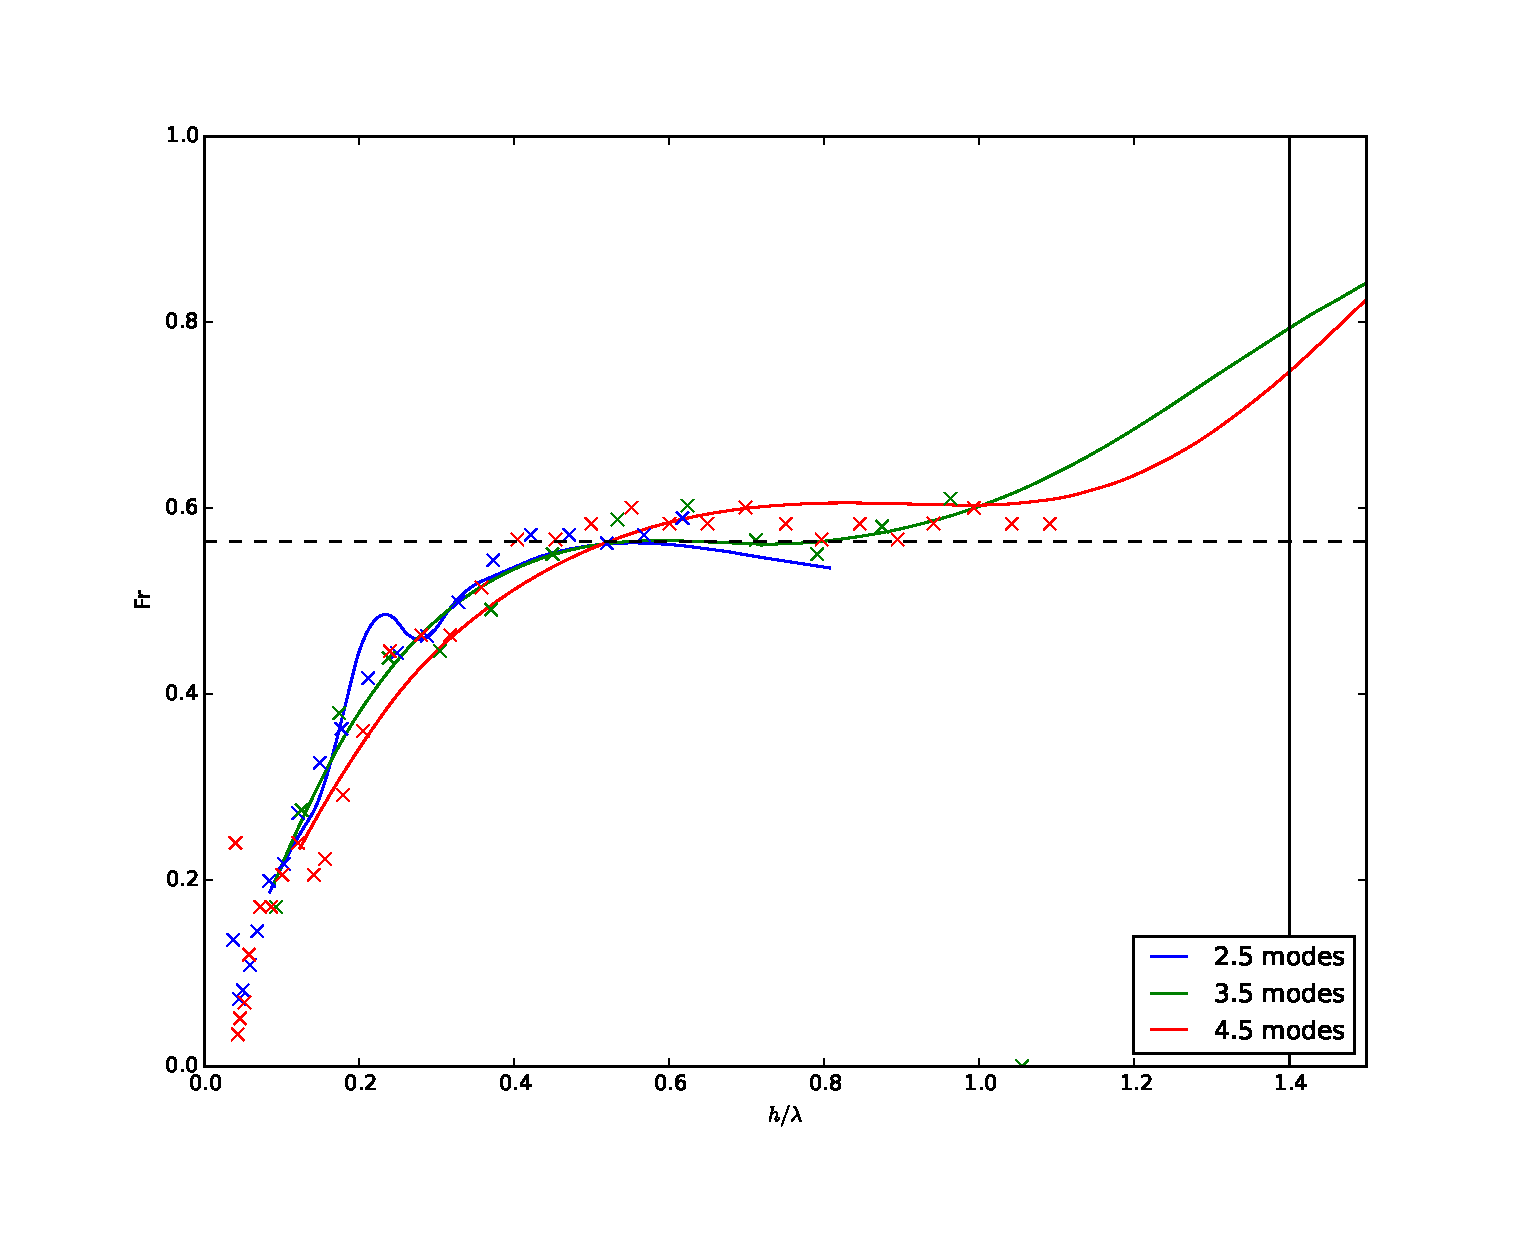
\includegraphics[width=\textwidth]{plts/Fr}
\caption{ \flabel{froude} 
Froude number vs.\ height, non-dimensionalized by the wavelength.
Lines are the derivative of cubic splines through simulation outputs.
Points are from experiment via direct measurement of the bubble velocity~\cite{JacobsPrivate}.
The dotted horizontal line is positioned at Goncharov's theoretical value of $\pi^{-1/2}$~\cite{Goncharov2002}.
}
\end{figure}

\begin{figure}
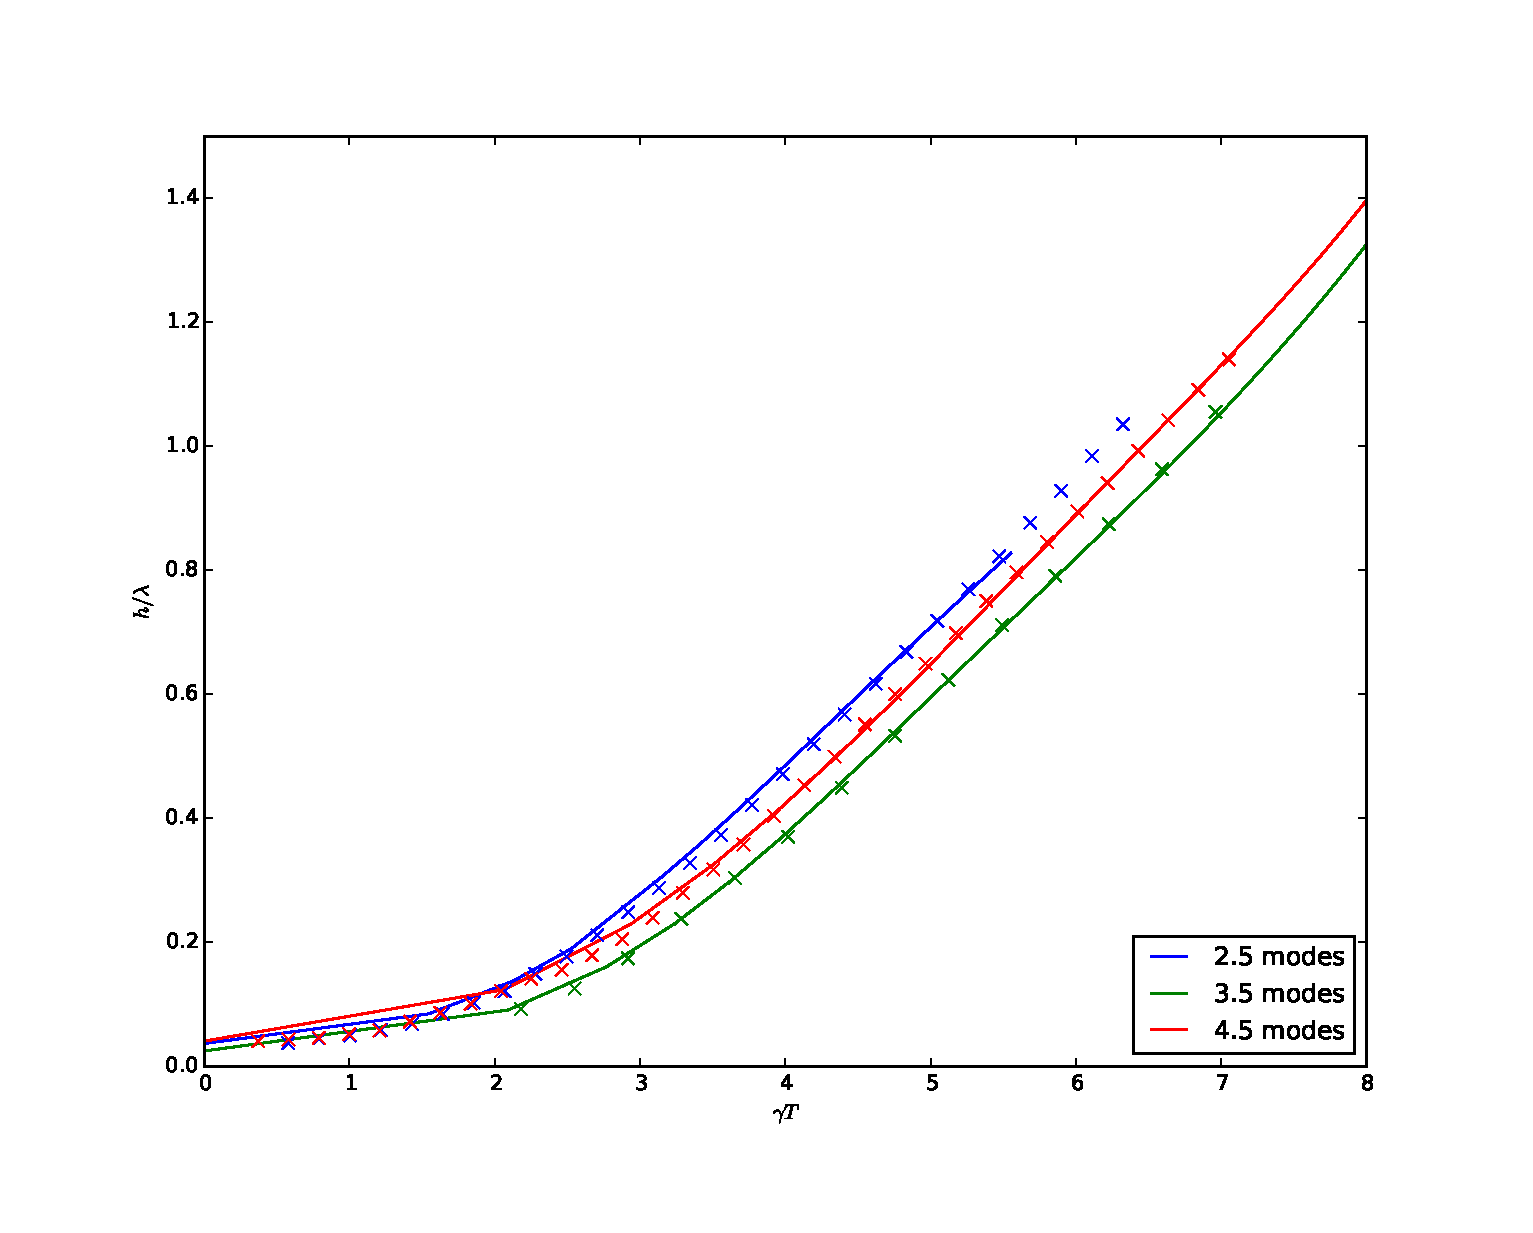
\includegraphics[width=\textwidth]{plts/aspect}
\caption{ \flabel{aspect} 
Bubble height vs.\ time, non-dimensionalized by the wavelength and linear growth rate, respectively.
Lines are cubic splines through simulation outputs.
Points are from experiment~\cite{JacobsPrivate}.
The points are shifted in time to minimize the square deviation from the spline summed over the plotted points.
}
\end{figure}

The experiments observe only the diagonal plane and measure the height with respect to the most internal bubble.
Therefore, we plot in \fref{froude} the non-dimensional velocity, i.e., the Froude number, of the central bubble alone:
\begin{equation}
	\text{Fr} = \frac{v}{\sqrt{ A g \lambda}}
\end{equation}
In each case, the simulation exhibits the same qualitative behavior as the experiment:
exponential growth saturating to a stagnation velocity around Goncharov's theoretical value of $\text{Fr} = \pi^{-1/2}$~\cite{Goncharov2002}.
In cases where the simulation and experimental data extend in time, the beginnings of re-acceleration are also seen.

The 2.5 mode case exhibits peculiar behavior, with two inflection points around aspect ratio $h / \lambda = 0.2$.
This is not an issue with the splines, as can be seen in \fref{aspect}, which plots the non-dimensional height vs.\ non-dimensional time without splines.
The 2.5 mode case, which has the highest Grashof and Schmidt numbers, went unstable.
Upon inspection, the 5\% filtering was unable to suppress the oscillations in the scalar field.
This simulation could be retried with greater resolution, but, given the stability of the 3.5 mode case, the computational cost would be up to 43$\times$ greater, which is why it was not repeated in this study.

\subsection{Extension}

Given the agreement between the simulations and the experiment, we can use the simulations to explore the flow in ways that are not readily accessible experimentally.
In this study, we extend the subject cases and analysis in three ways.
First, we calculate the height of each bubble in the tank individually and use the results to study finite size effects.
Second, we extend the 4.5 mode experiment by a factor of two in the vertical extent of the domain and simulation time to delay interaction with the top boundary and reach later times and larger bubble heights.
Finally, we consider the span-wise, vs.\ stream-wise, flow by taking slices of the midplane and observing pressure driven secondary flows.
These three extensions are a small sample of the types of observations that are available numerically.

\subsubsection{Wall effects}

\begin{figure*}
\begin{subfigure}[b]{0.5\textwidth}
  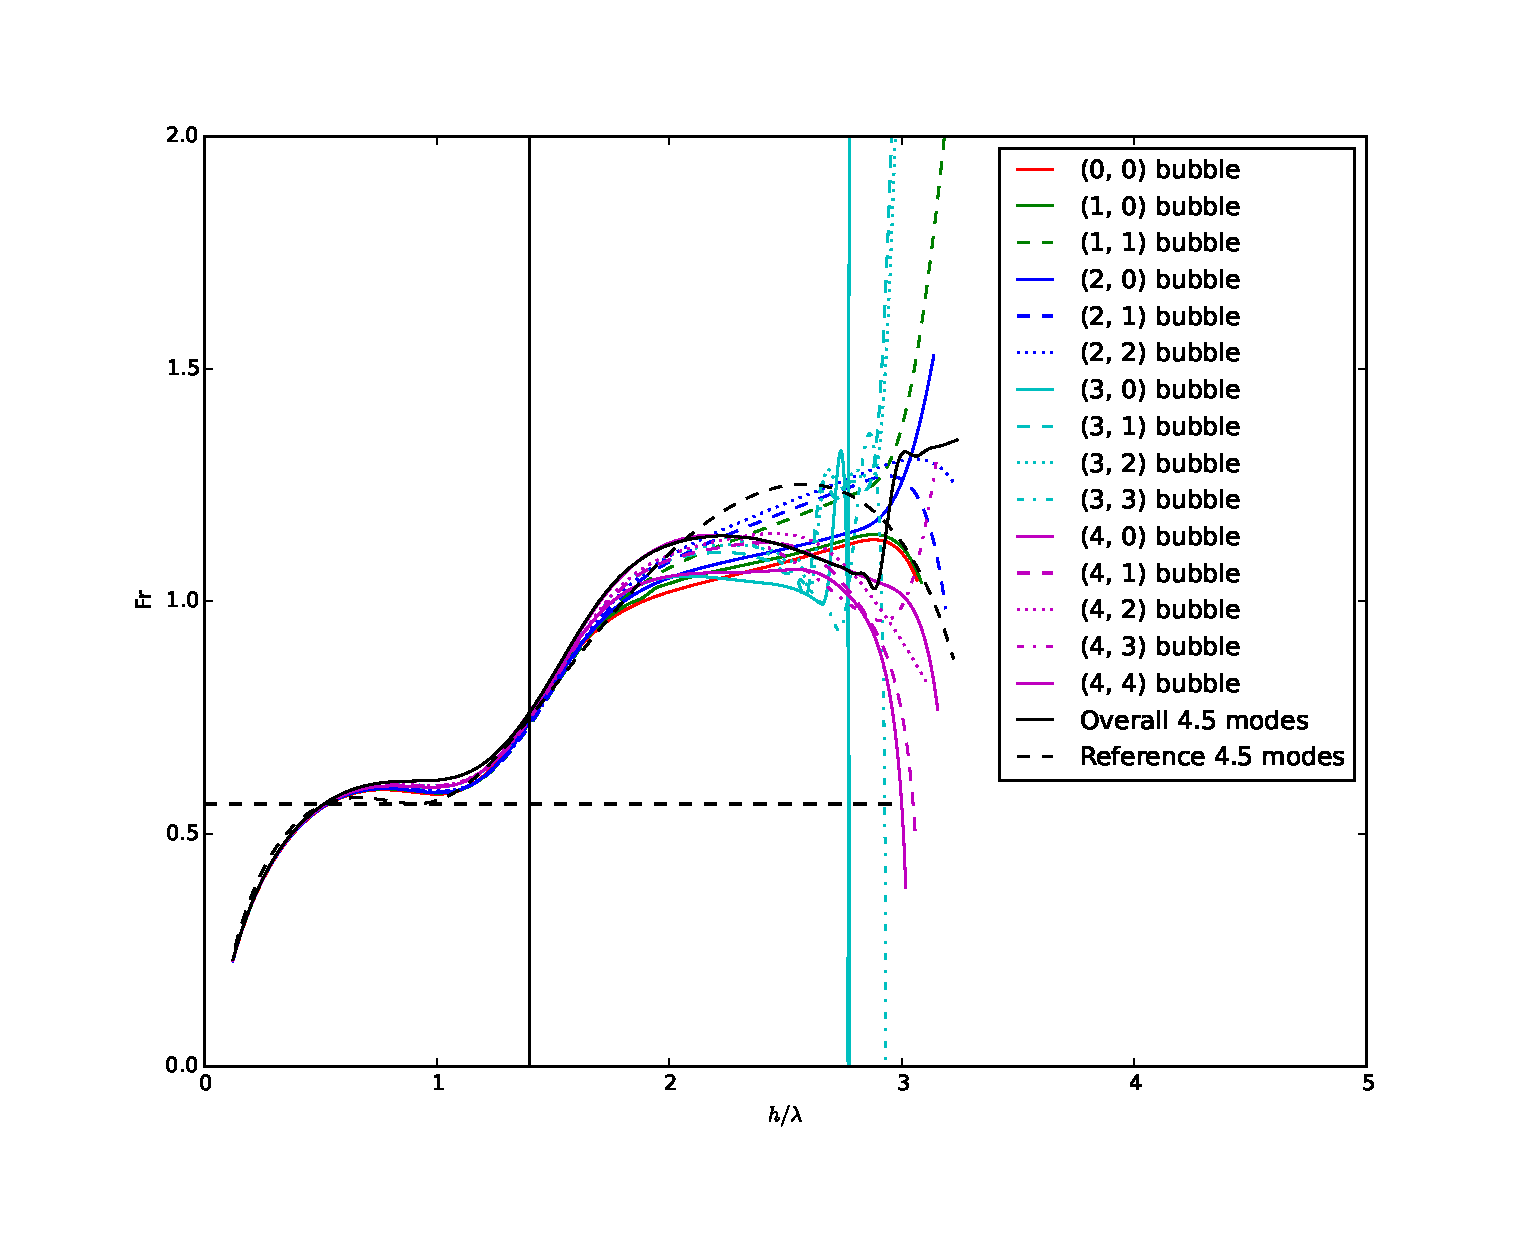
\includegraphics[width=\textwidth]{plts/walls_Fr}
\end{subfigure}
\begin{subfigure}[b]{0.5\textwidth}
  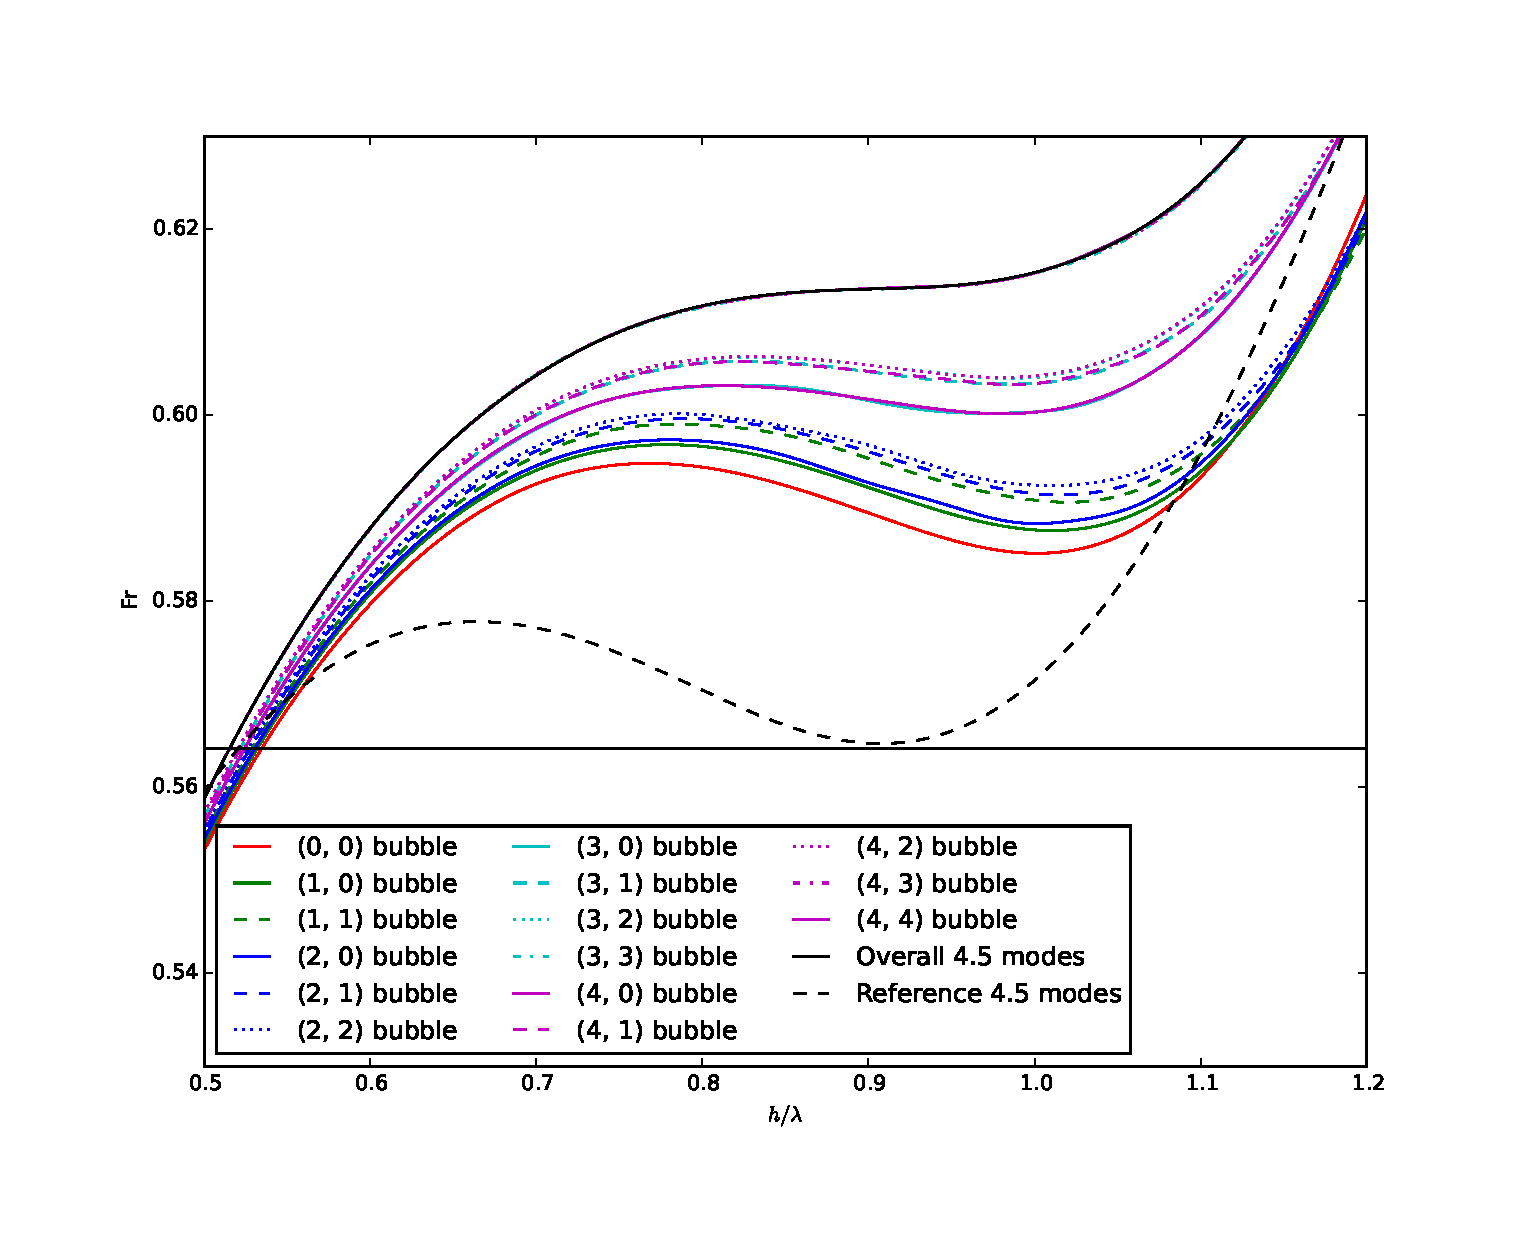
\includegraphics[width=\textwidth]{plts/walls_Fr_zoom}
\end{subfigure}
\caption{ \flabel{froude_wall} 
Froude number as a function of height, non-dimensionalized by the wavelength, by bubble in the 4.5 mode simulation.
Solid line is from the height defined as the maximum taken over the entire span-wise domain.
Dotted line is the periodic reference calculation.
}
\end{figure*}

\begin{figure*}
\begin{subfigure}[b]{0.5\textwidth}
  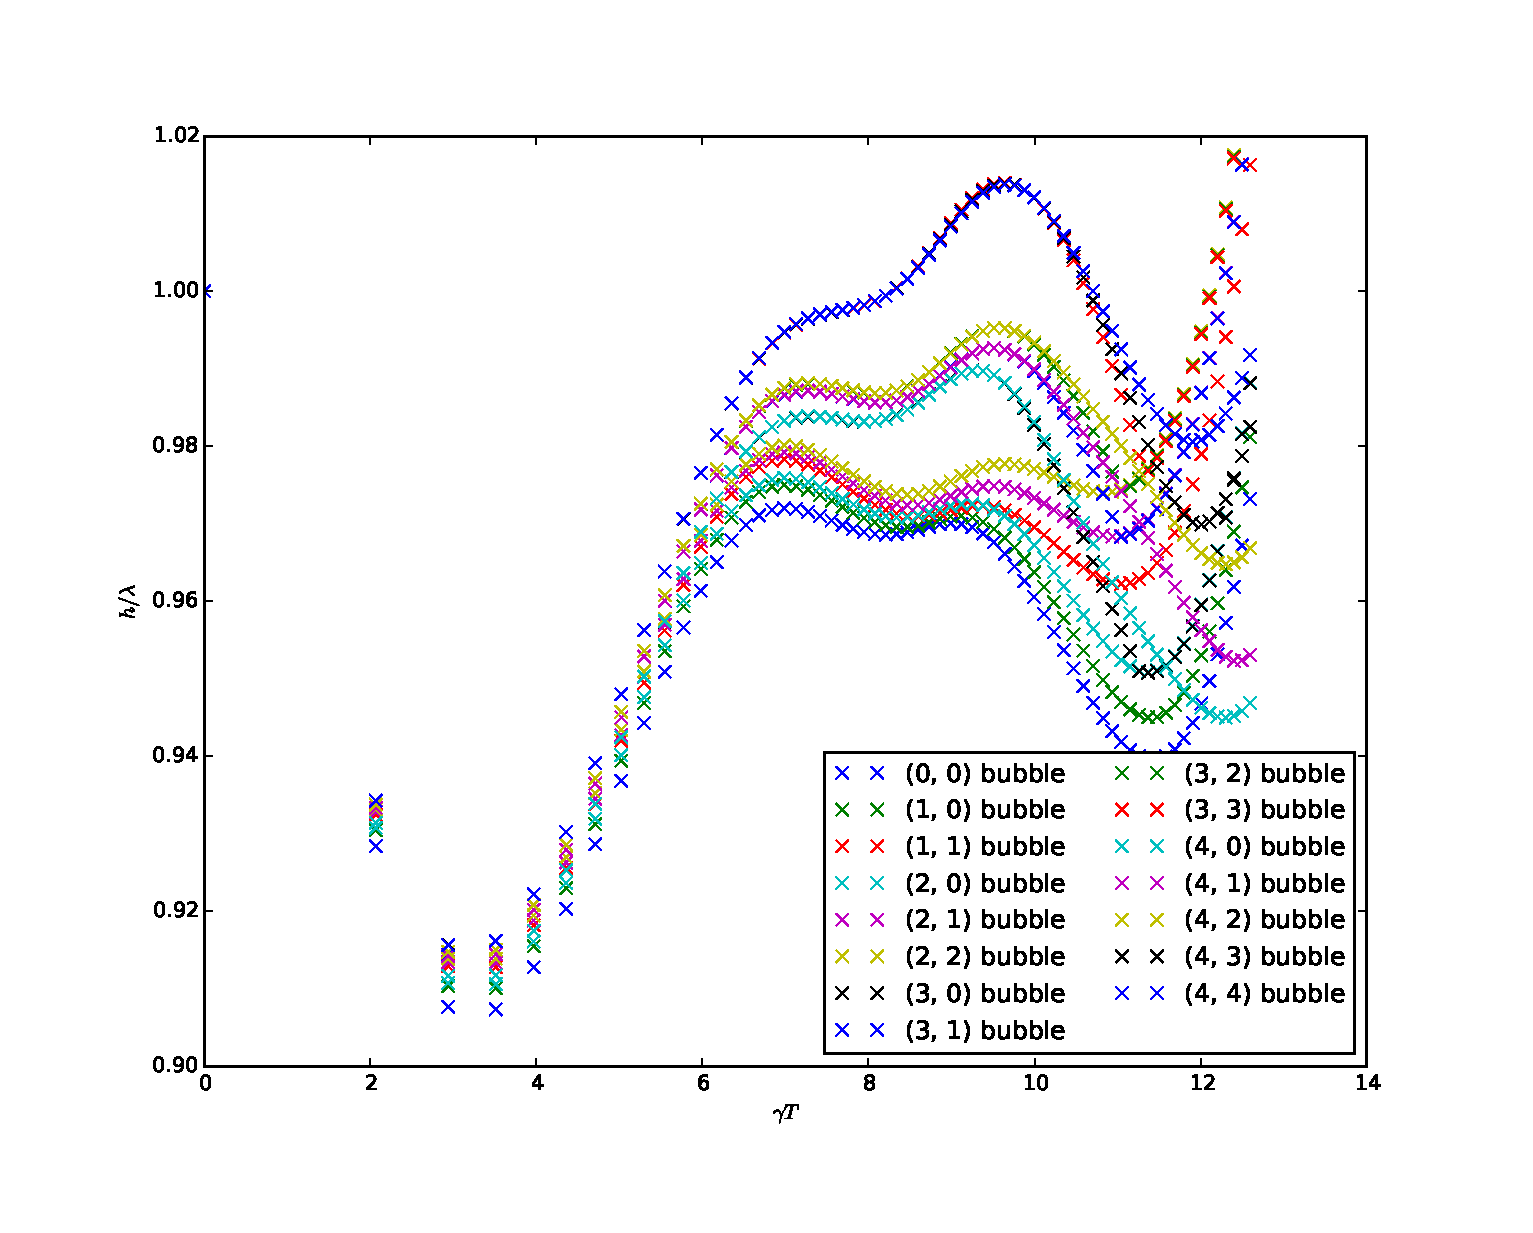
\includegraphics[width=\textwidth]{plts/walls_h}
\end{subfigure}
\begin{subfigure}[b]{0.5\textwidth}
  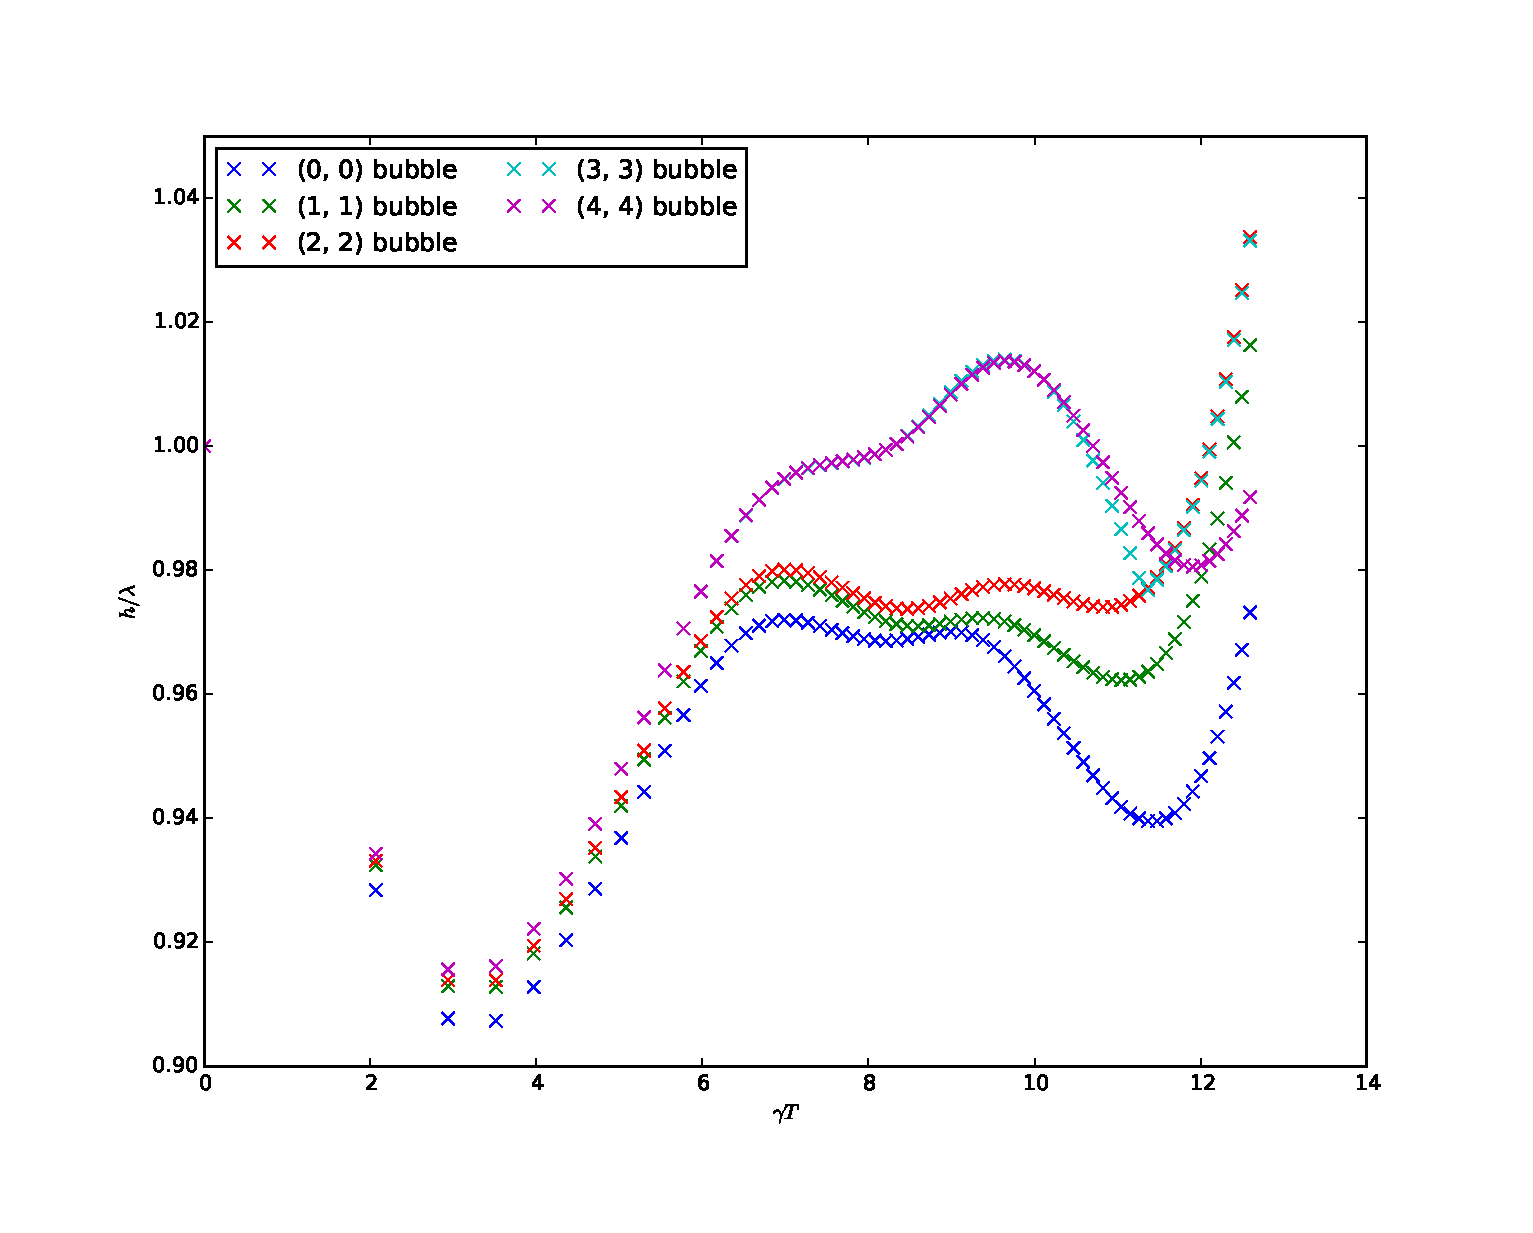
\includegraphics[width=\textwidth]{plts/walls_h_diag}
\end{subfigure}
\caption{ \flabel{ratio_wall}
Ratio of wall-bounded bubble height to periodic bubble height in the 4.5 mode simulation.
}
\end{figure*}

\begin{figure*}
\begin{subfigure}[b]{0.49\textwidth}
  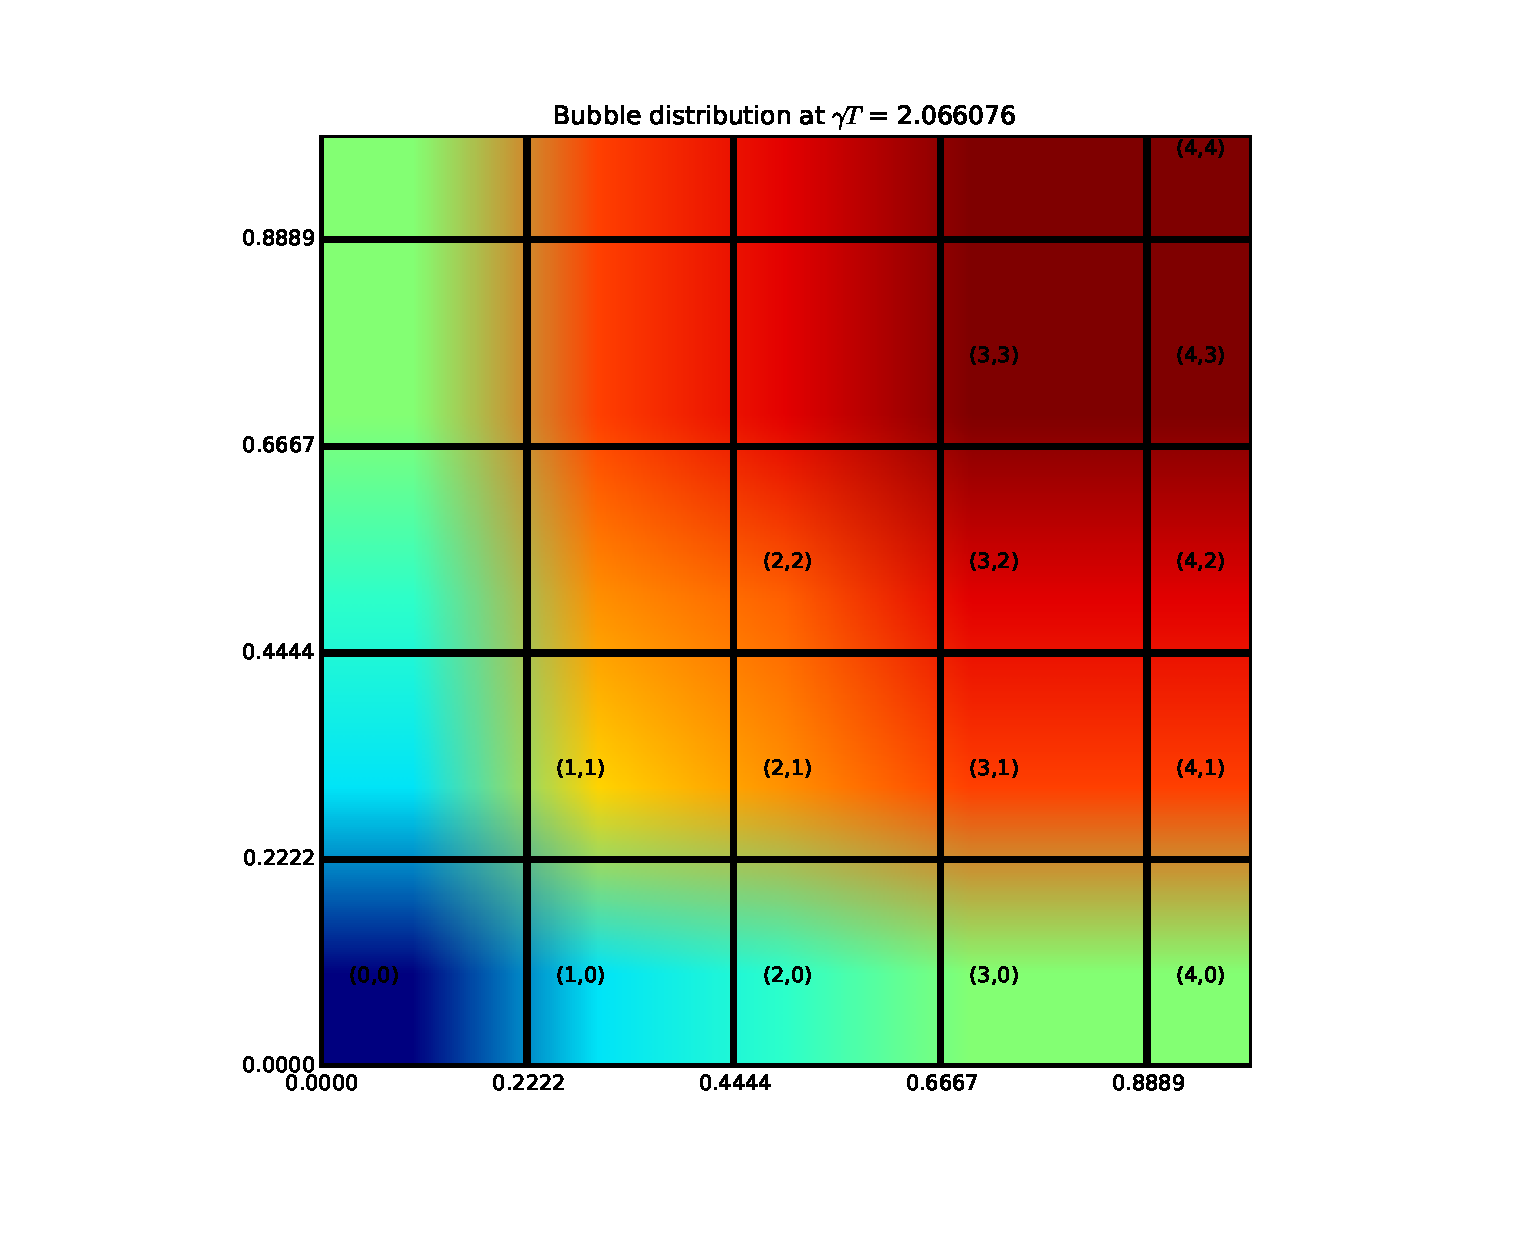
\includegraphics[width=\textwidth]{figs/spatial_bubble-1}
\end{subfigure}
\begin{subfigure}[b]{0.49\textwidth}
  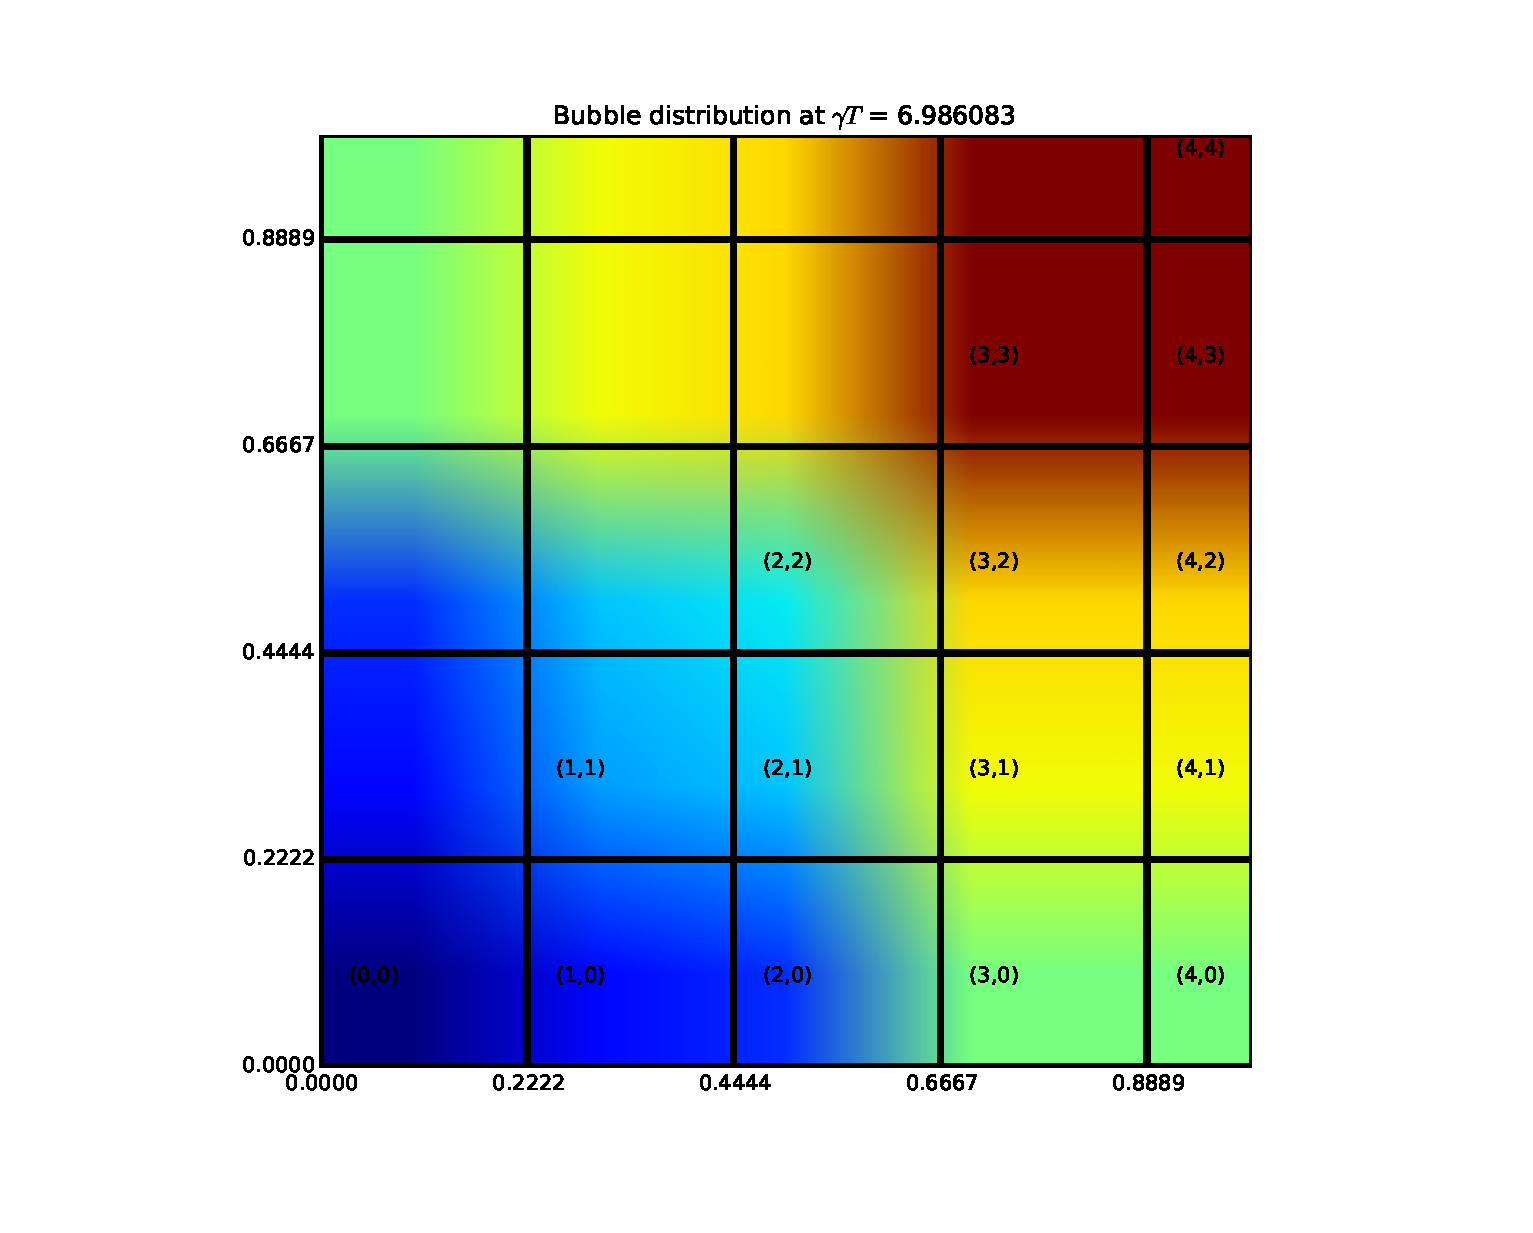
\includegraphics[width=\textwidth]{figs/spatial_bubble-17}
\end{subfigure}
\begin{subfigure}[b]{0.49\textwidth}
  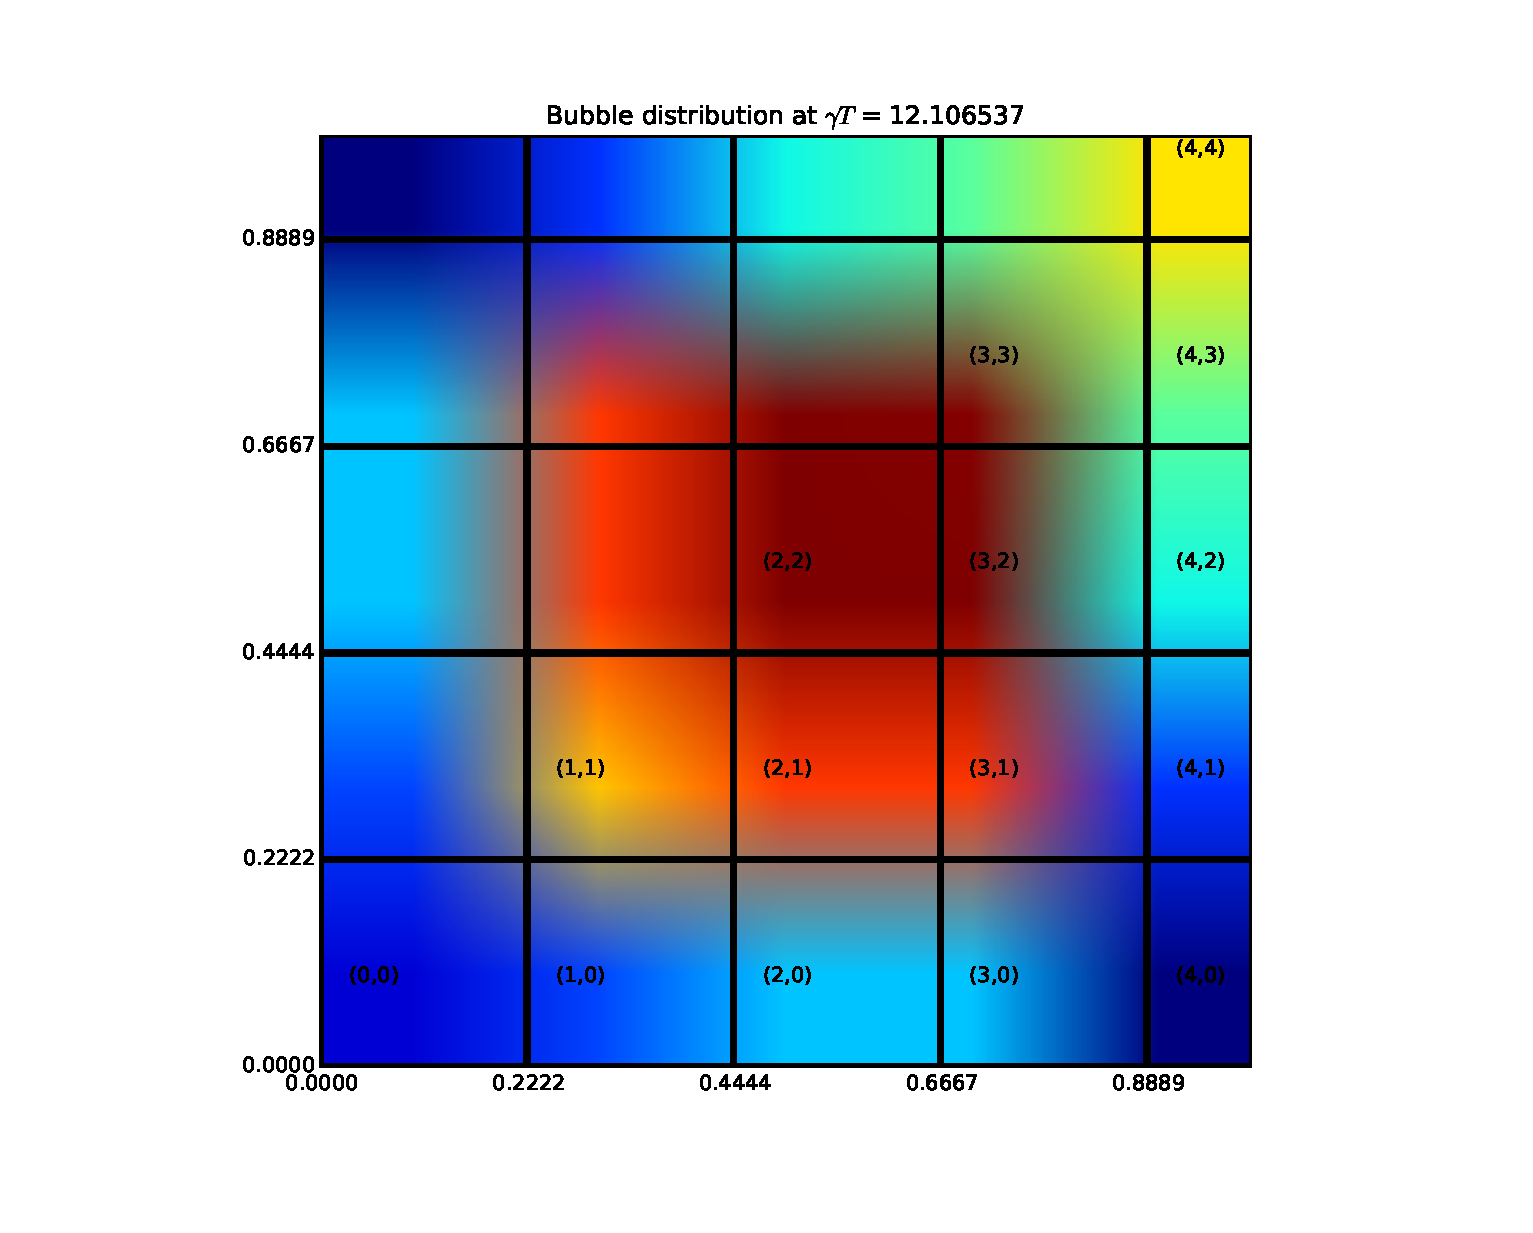
\includegraphics[width=\textwidth]{figs/spatial_bubble-59}
\end{subfigure}
\caption{ \flabel{bubble_slice}
Spatial distribution of bubble heights at three times, with red denoting greater bubble heights and blue denoting lesser bubble heights.
The first time is when the ratio of the wall-bounded to periodic bubble height is at a minimum, which is during the transition from linear to non-linear growth; a long wavelength mode is seen across the diagonal.
The second time is taken from the stagnation phase; the long wavelength mode is still present.
The third time is taken from the end of the simulation; the central bubbles are being squeeze significantly ahead of the bubbles near the wall.
}
\end{figure*}

The individual bubble heights for the $4.5$ mode case are computed as in \eref{h_exp}, but restricted to the span-wise domain nearest to the bubble tip, which is marked in \fref{ic}.
The bubble Froude numbers are plotted in \fref{froude_wall}, alongside the aggregate and purely periodic values.

There are at least three mechanisms by which the walls divert the flow from its fully-periodic preference.
The first is that the no-slip boundaries that pass along the diagonal of the boundary bubbles and spikes create a boundary layer that viscously damps vertical flow.
The second is that the pressure gradient from the boundary layer pushes the boundary bubbles and spikes towards the interior of the domain.
These two effects have been studied independently in the context of multi-phase bubbles rising near walls~\cite{Takemura2002}, and are characterized as wall drag and lift forces.
Finally, the finite nature of the span-wise lattice of bubbles and spikes, coupled with the vertical symmetry condition that the total bubble volume must equal the total spike volume, breaks one of the 4-fold symmetries of the infinite cubic lattice causing a local aggregation of spikes in the $(0,0)$ corner and of bubbles in the $(4,4)$ corner.
The local aggregation sets up one low-amplitude long-wavelength mode across the diagonal.

These three mechanisms promote and penalize the growth of different bubbles in the finite lattice, allowing us to infer the relative magnitudes of the effects based on the performance of the bubbles compared to their periodic counterparts.
The wall drag penalizes the growth of bubbles that contain a boundary: the bubbles in the 4th column.
Because the effect also penalizes the growth of the spikes that contain boundaries, it should encourage the growth of the bubbles adjacent to those spikes: those in the 0th row.
The effect should alternate and diminish towards the interior of the domain.
The wall lift pushes bubbles and spikes at the boundary towards the interior.
This reduces the form drag on the interior bubbles by increasing the pressure on their trailing edges.
When adjacent bubbles actually touch, skin drag is also reduced.
Overall, wall lift promotes the growth of the interior bubbles.
Finally, the long-wavelength mode promotes growth of bubbles in the bubble heavy corner and penalizes growth of bubbles in the spike heavy corner.

The spatial distribution of the bubble heights can be seen in \fref{bubble_slice} and the heights relative to the periodic bubble can be seen in \fref{ratio_wall}.
At moderate times, the $(4,4)$ bubble leads and the $(0,0)$ bubble trails, indicating that the long-wavelength mode due to symmetry breaking is the dominant effect.
Additionally, all of the bubbles under-perform their periodic counterpart, indicating that the wall drag has damped the overall flow but with less spatial dependence than the long-wavelength mode.
At late times, the central $(2,2)$, $(2,1)$  bubbles are accelerated while the edge bubbles break down, indicating the growing importance of the wall lift effect.
The wall lift ultimately leads to bubble collisions that destroy the bubble lattice, enhance mixing, and break down the flow.

\subsubsection{Late-time behavior}

\begin{figure*}
\begin{subfigure}[b]{0.5\textwidth}
  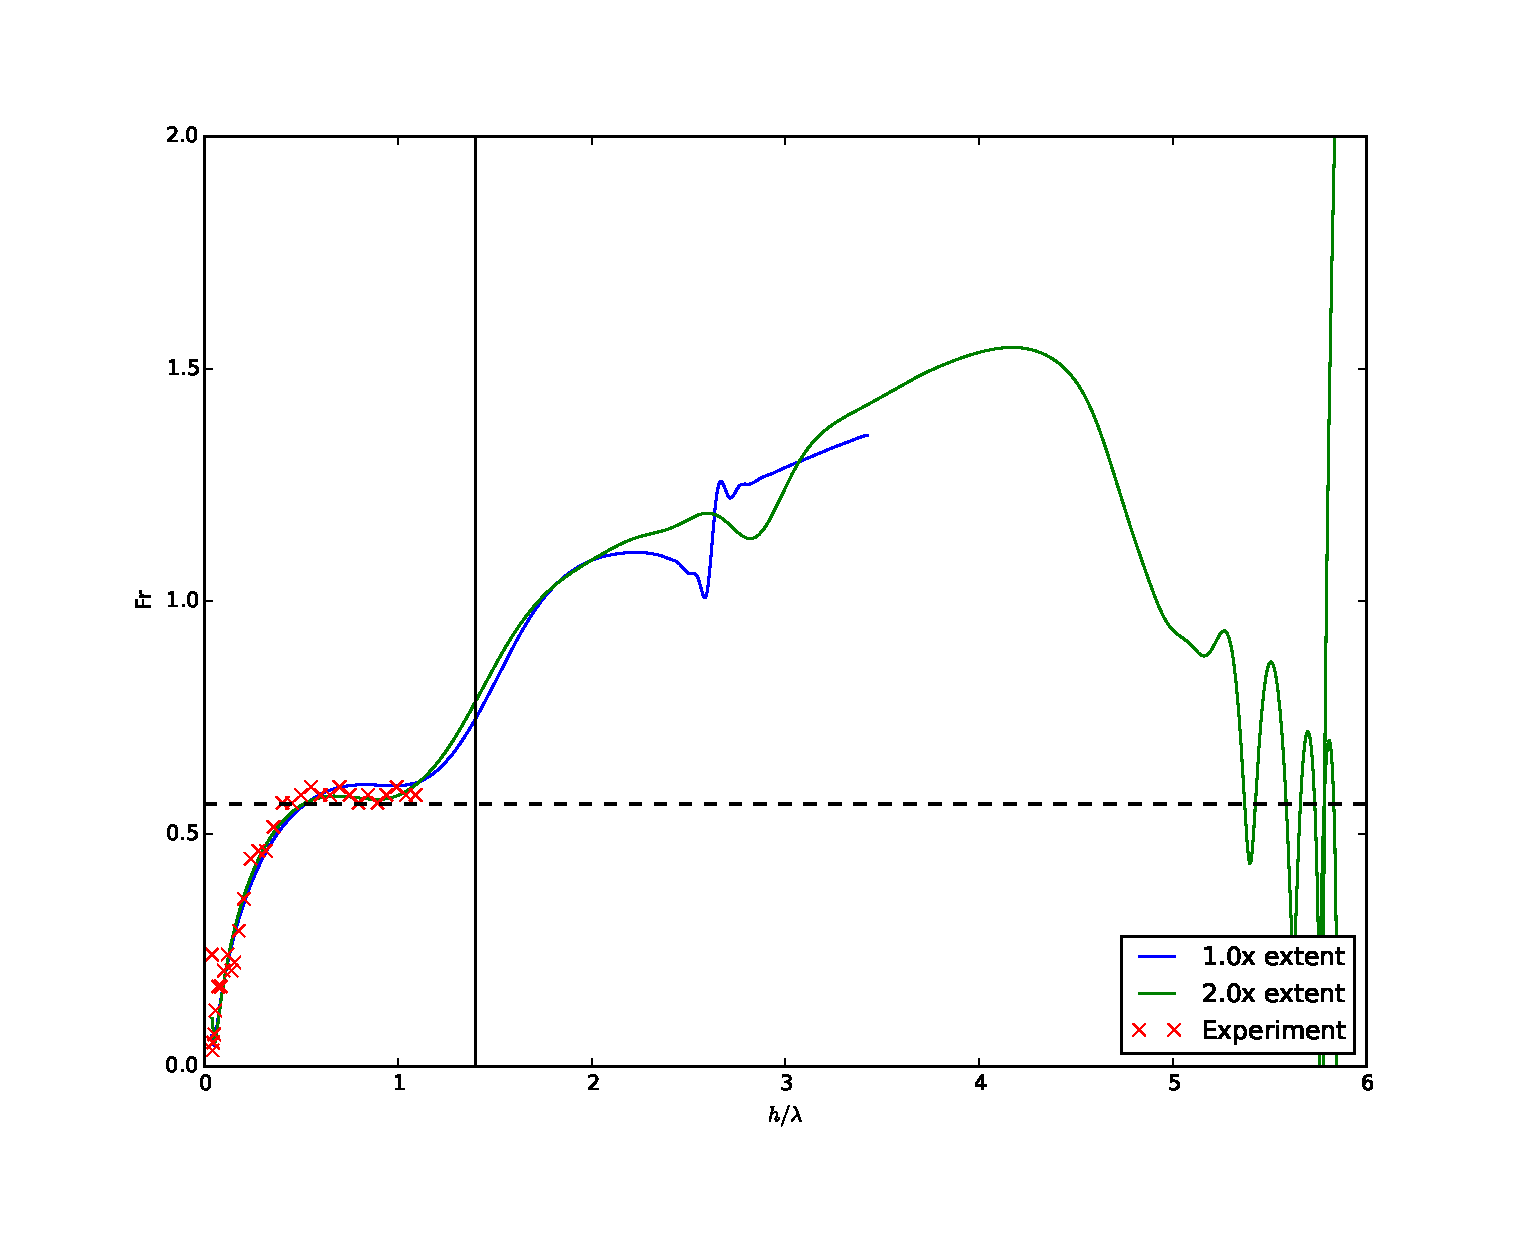
\includegraphics[width=\textwidth]{plts/Fr_long}
\end{subfigure}
\begin{subfigure}[b]{0.5\textwidth}
  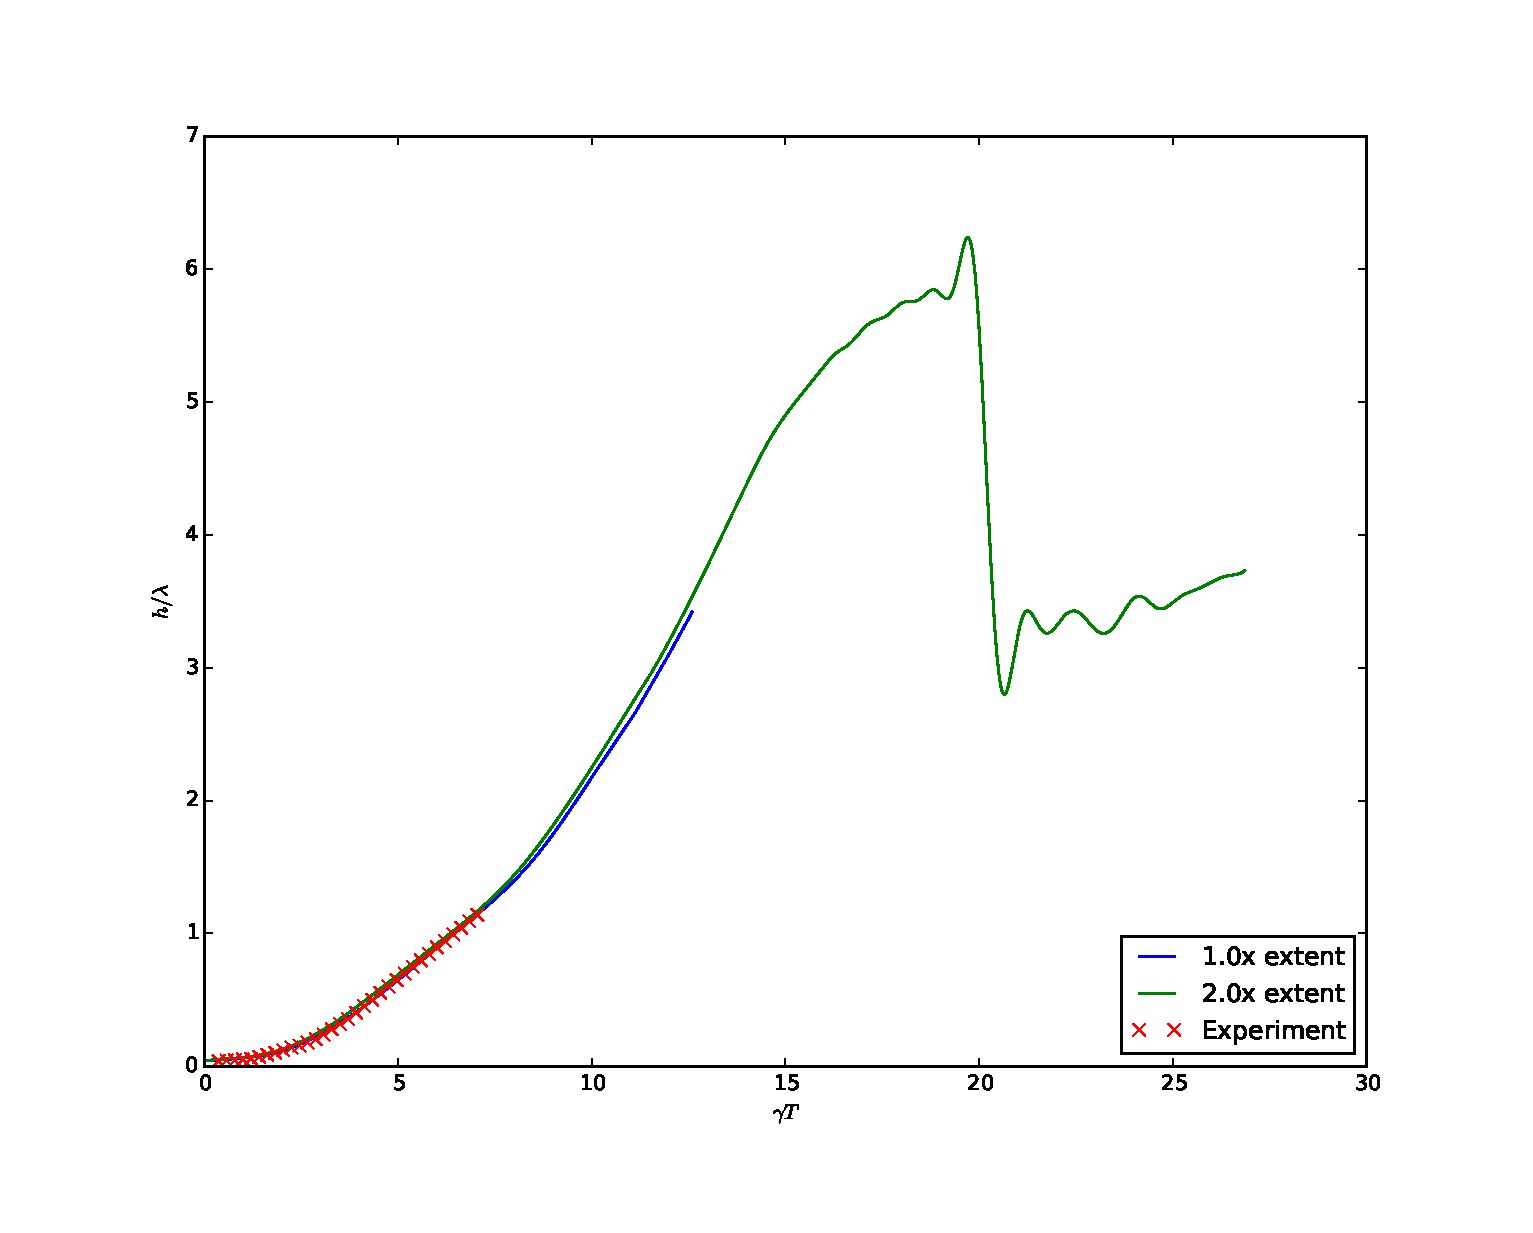
\includegraphics[width=\textwidth]{plts/aspect_long}
\end{subfigure}
\caption{ \flabel{long_dynamics}
Bubble velocity and bubble height vs.\ time, non-dimensionalized by the wavelength and linear growth rate, for 4.5 mode simulations and experiment.
Lines are from simulation output, one case with the same vertical extent as the simulation and in the other with twice that vertical extent.
Points are from experiment via direct measurement of the bubble velocity and bubble height.
The dotted horizontal line is positioned at Goncharov's theoretical value of $\pi^{-1/2}$~\cite{Goncharov2002}.
The solid vertical line marks the greatest bubble height reached in any of the experiments by Wilkinson and Jacobs~\cite{Wilkinson2007}.
}
\end{figure*}

\begin{figure*}
\begin{subfigure}[b]{0.32\textwidth}
  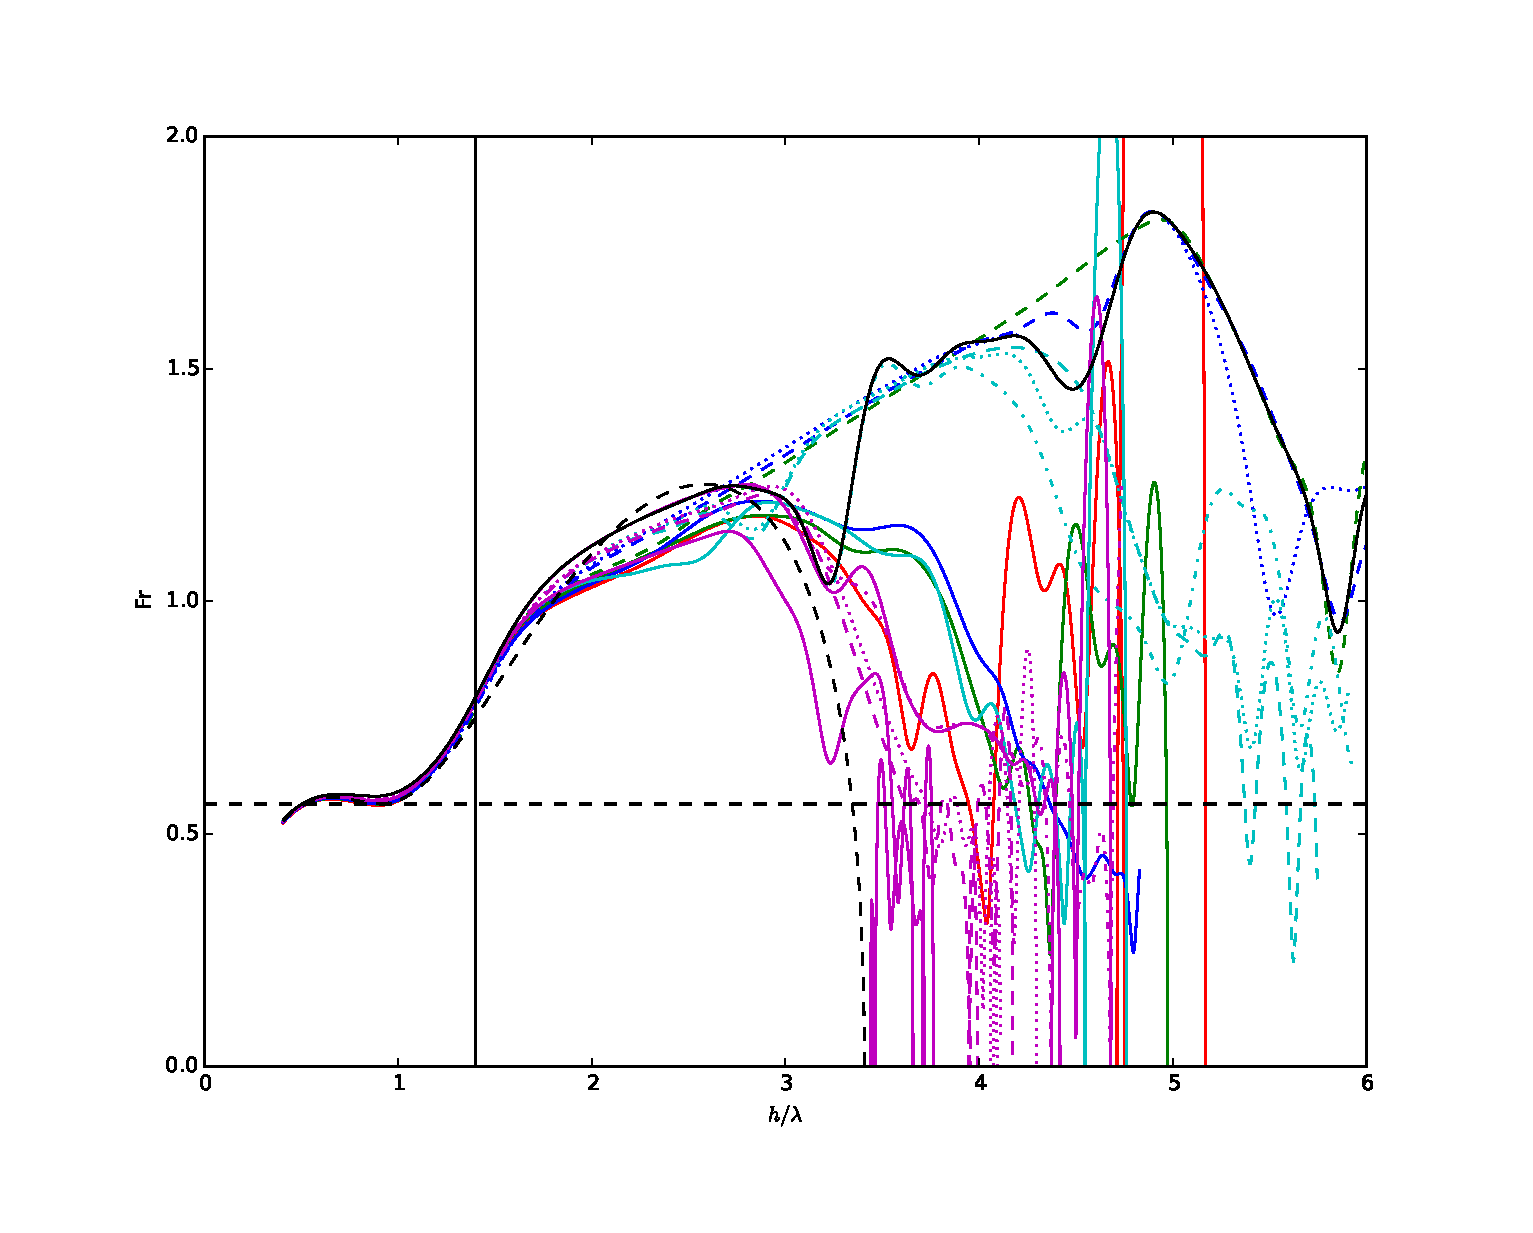
\includegraphics[width=\textwidth]{plts/Fr_long_walls}
\end{subfigure}
\begin{subfigure}[b]{0.32\textwidth}
  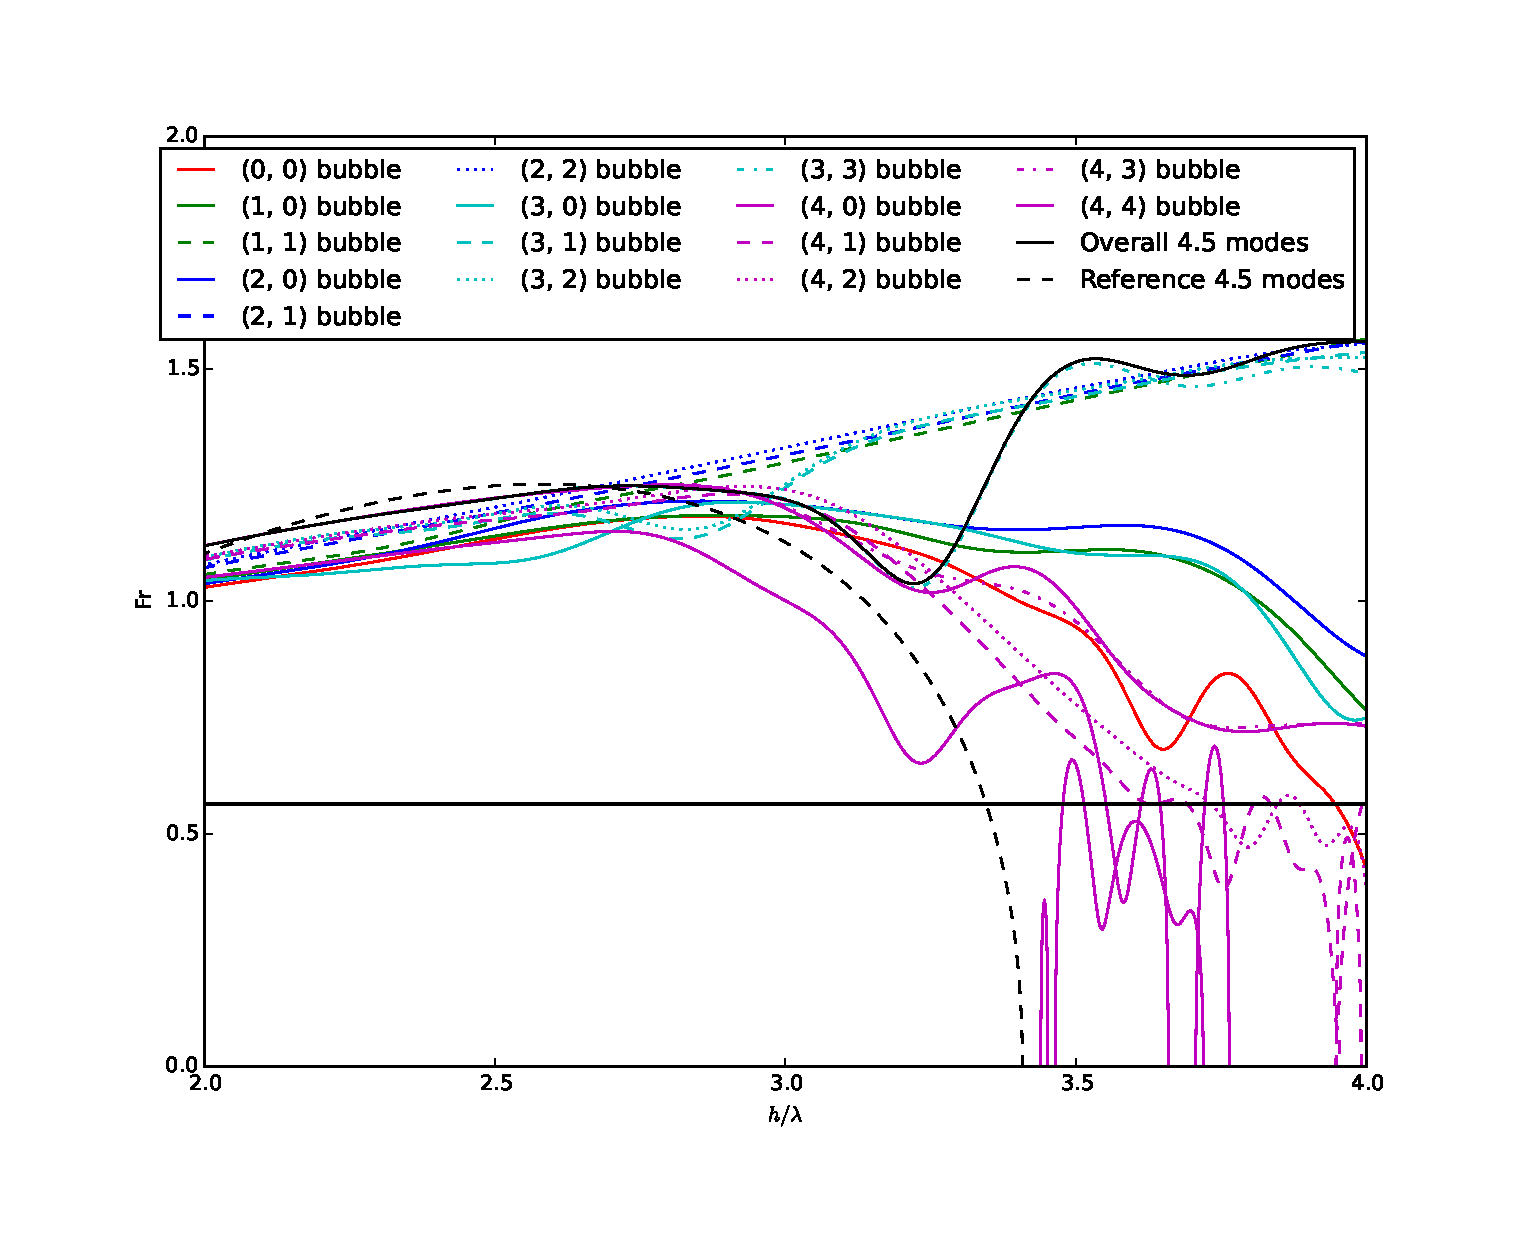
\includegraphics[width=\textwidth]{plts/Fr_long_walls_zoom1}
\end{subfigure}
\begin{subfigure}[b]{0.32\textwidth}
  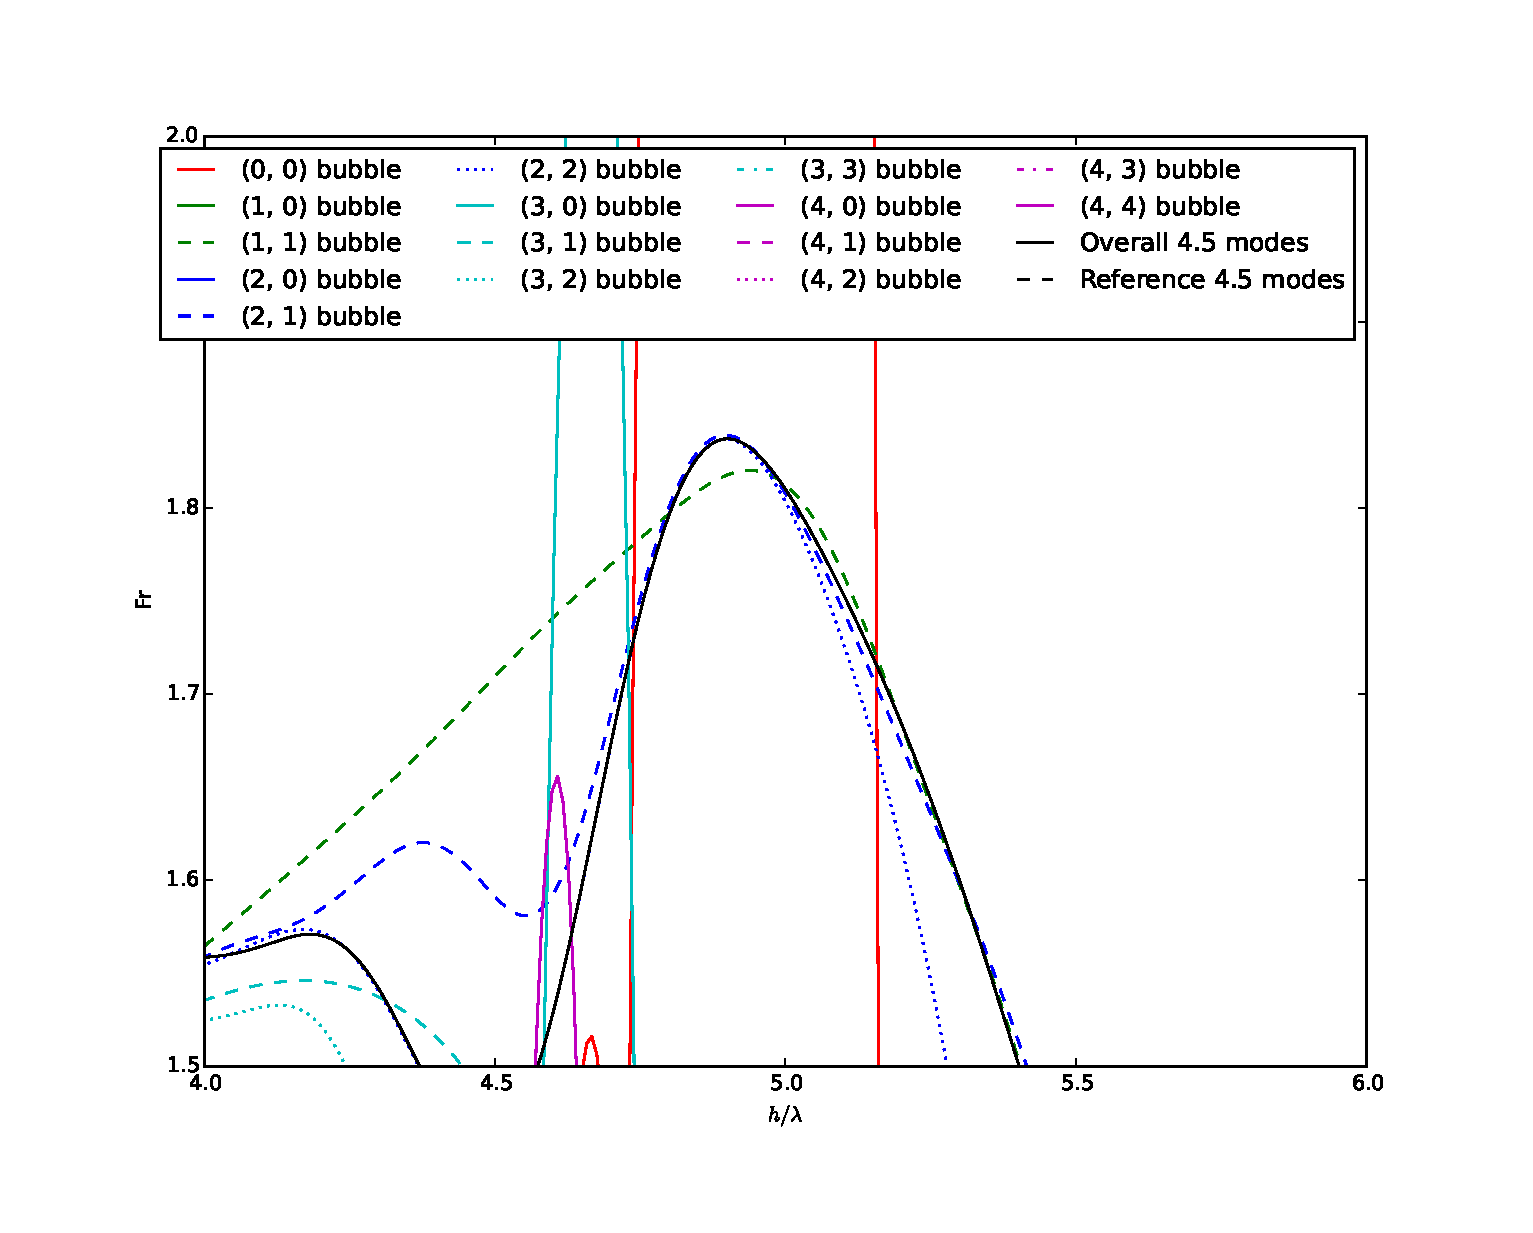
\includegraphics[width=\textwidth]{plts/Fr_long_walls_zoom2}
\end{subfigure}
\caption{ \flabel{long_wall_dynamics}
Froude number as a function of height, non-dimensionalized by the wavelength, by bubble in the 4.5 mode simulation with extended vertical extent.
Solid line is from the height defined as the maximum taken over the entire span-wise domain.
Dotted line is the periodic reference calculation.
The dotted horizontal line is positioned at Goncharov's theoretical value of $\pi^{-1/2}$~\cite{Goncharov2002}.
The solid vertical line marks the greatest bubble height reached in any of the experiments by Wilkinson and Jacobs~\cite{Wilkinson2007}.
}
\end{figure*}


The 4.5 mode simulation was repeated with twice the vertical extent and simulation time.
Additionally, the Schmidt number was increased from 1 to 3.5 to reduce late-time mixing not present in high Schmidt number experiments.
\fref{long_dynamics} compares the short unit-Schmidt and long moderate-Schmidt trajectories, which are widely in agreement.
The reduction in bubble acceleration around aspect ratio $h/\lambda = 2$ is present in both the short and the long simulations, so it is unlikely to be due to the vertical domain boundaries.
It is not, however, present in the periodic calculation, so it could be a wall effect.

\fref{long_wall_dynamics} mimics \fref{froude_wall} but for the late-time case.
The periodic reference trajectory, calculated with the original domain size, rapidly decays after reaching a maximum around aspect ratio $h/\lambda = 2.5$ due to interactions with the top of the domain.
Its maximum Froude number is around 1.2, consistent with previous calculations.
The central bubbles in the extended late-time run continue to experience constant acceleration past aspect ratio 3 and Froude number 1.2, with the $(1,1)$ bubble continuing to aspect ratio 5 and Froude number 1.8.

The decay of the velocity of the periodic reference bubble around $h/\lambda = 2.5$ suggests the late-time simulations would interact with the top boundary around $h/\lambda = 5$.
In fact, this is exactly when the $(1,1)$ and $(2,2)$ bubbles begin to decay.
However, the bubbles closer to the boundaries break down much earlier.
The $(4,4)$ bubble, for example, reaching maximum Froude number around $h/\lambda = 2.75$.
We can infer that the wall lift that drives the boundary bubbles into the interior bubbles destroys the periodic ordering.
It is not clear if the decay of the interior bubbles at $h/\lambda = 5$ is due to the top boundary or the wall lift destroying the periodic ordering.

\subsubsection{Secondary flow}

\begin{figure*}
\begin{subfigure}[b]{0.32\textwidth}
  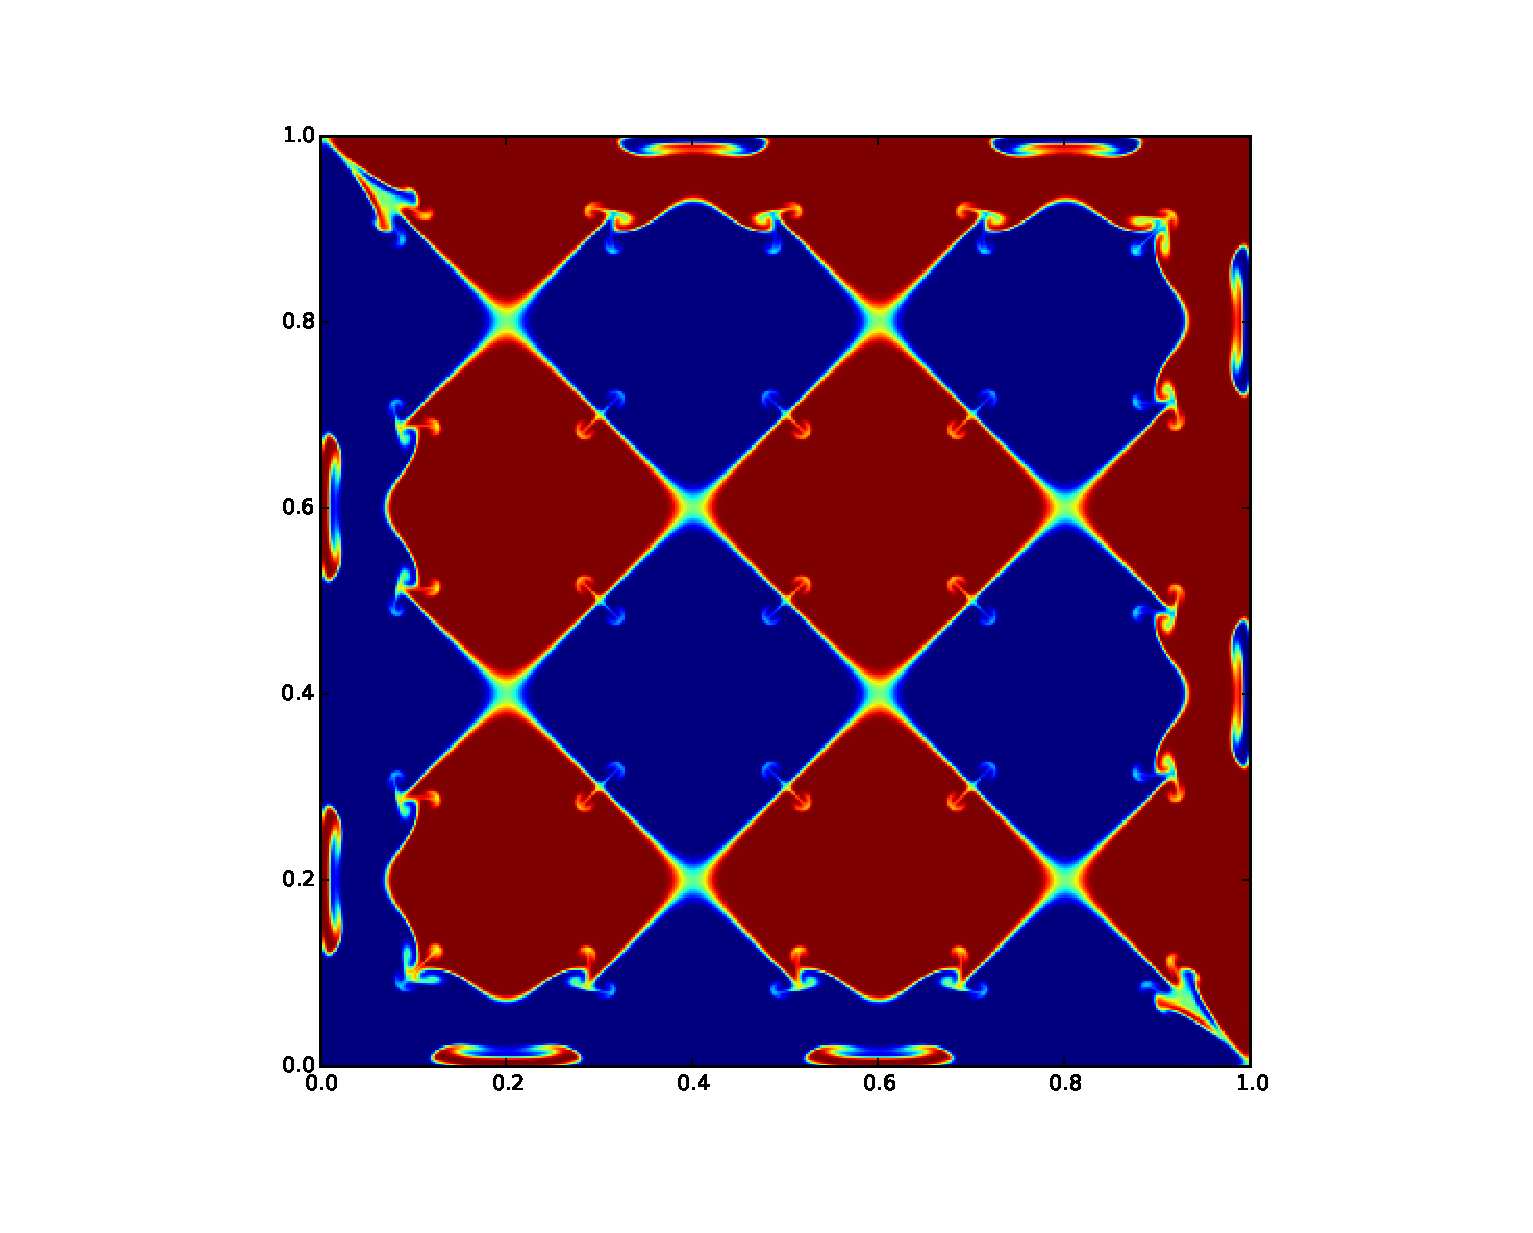
\includegraphics[width=\textwidth]{figs/scalar-25-20}
\end{subfigure}
\begin{subfigure}[b]{0.32\textwidth}
  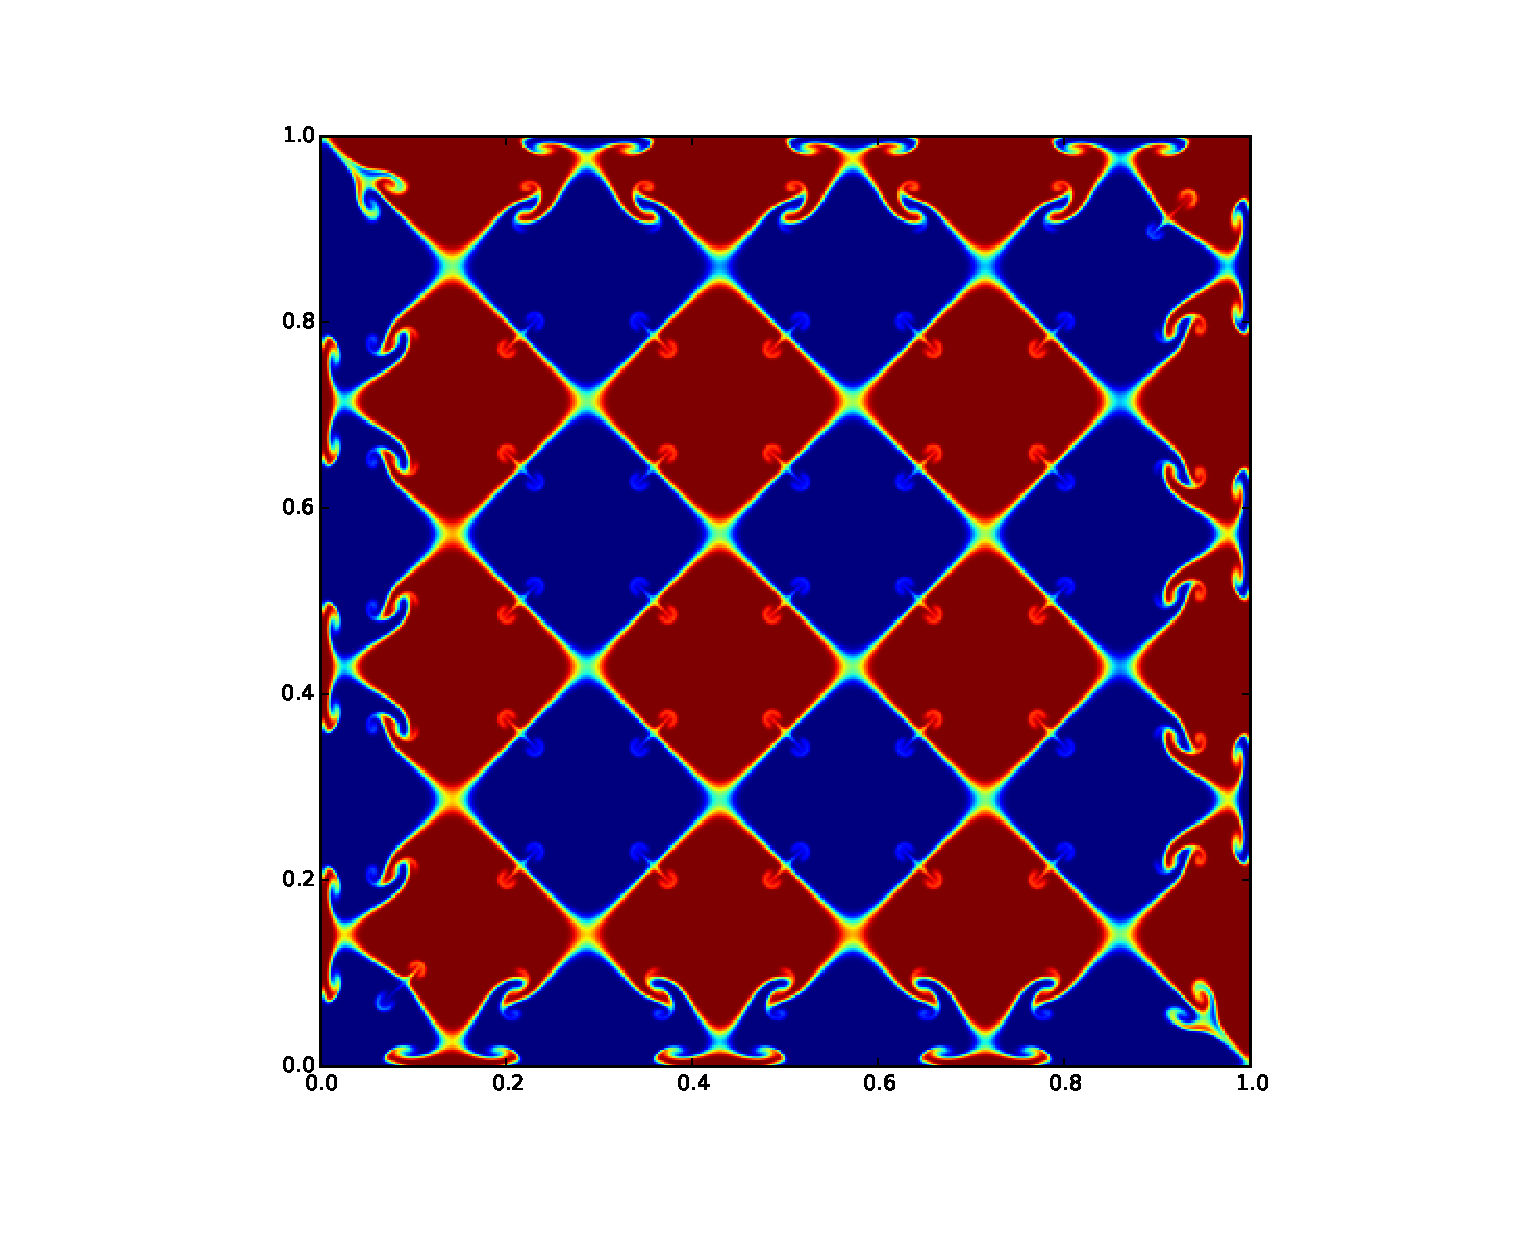
\includegraphics[width=\textwidth]{figs/scalar-35-20}
\end{subfigure}
\begin{subfigure}[b]{0.32\textwidth}
  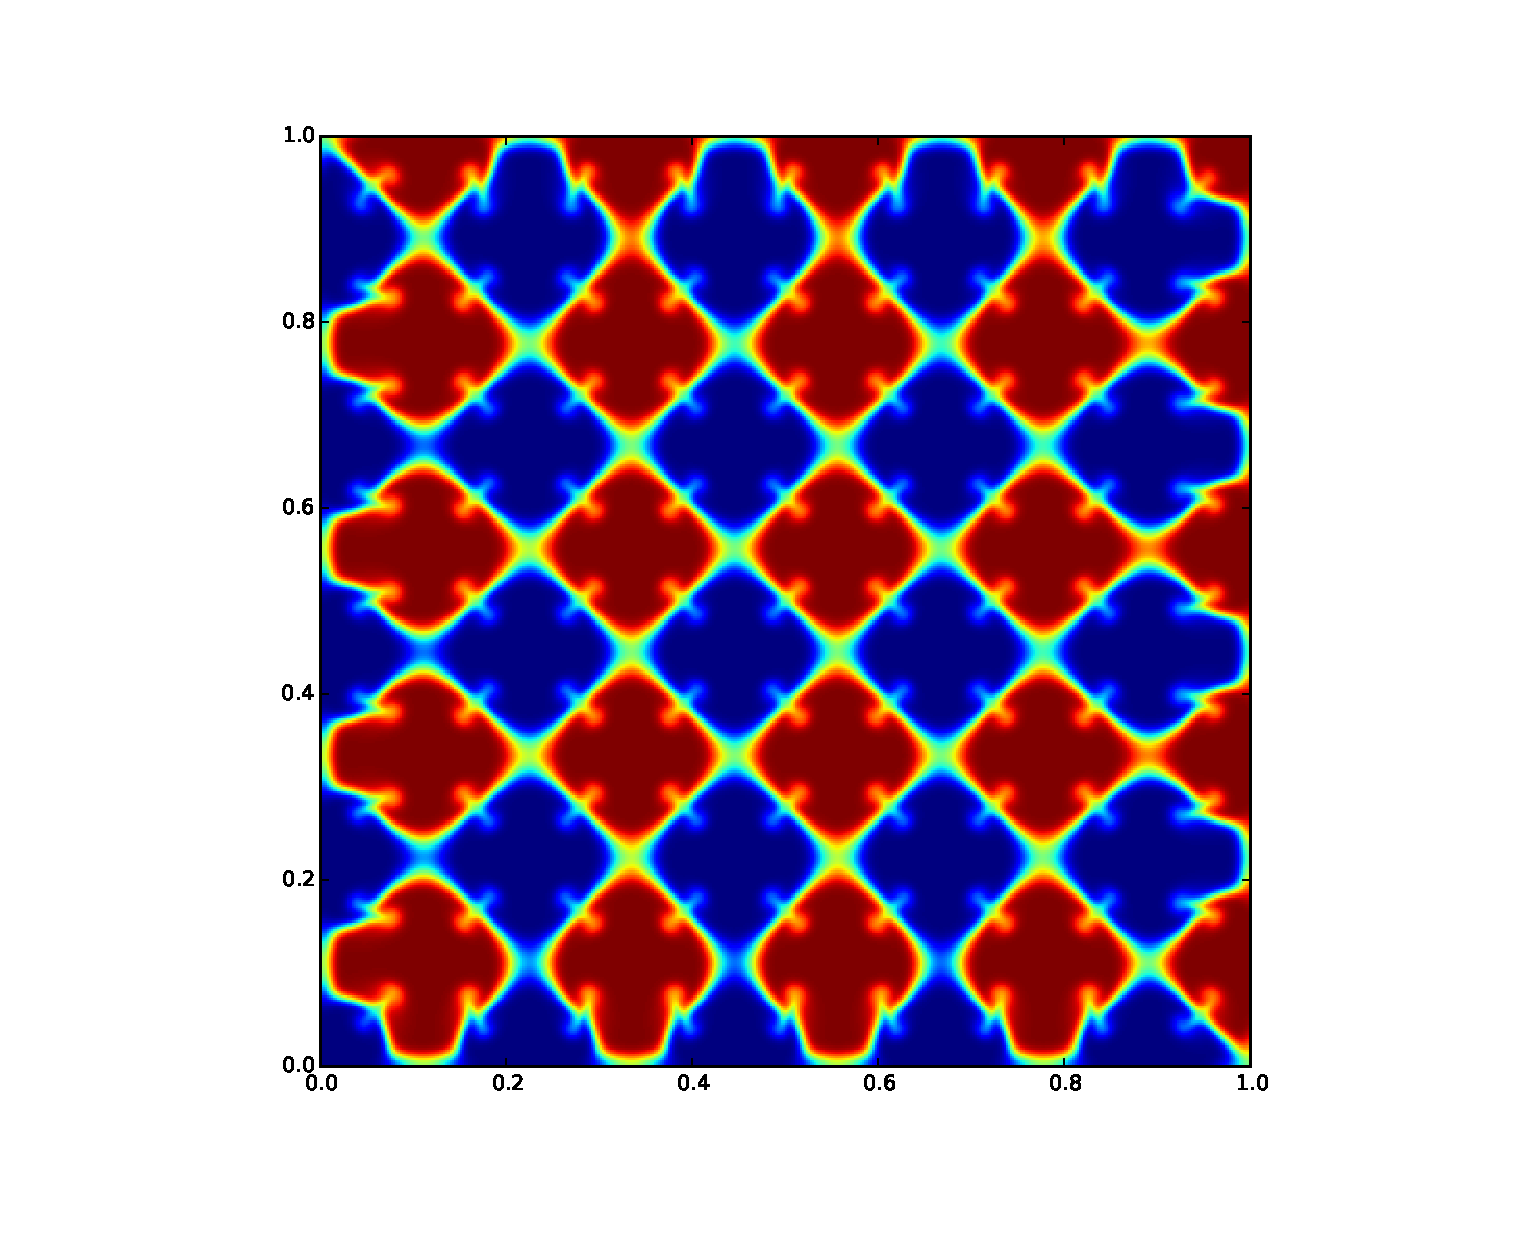
\includegraphics[width=\textwidth]{figs/scalar-45-20}
\end{subfigure}
\caption{ \flabel{phixy}
Scalar field in the horizontal mid-plane for 2.5, 3.5, and 4.5 mode simulations.
}
\end{figure*}



\begin{figure*}
\begin{subfigure}[b]{0.32\textwidth}
  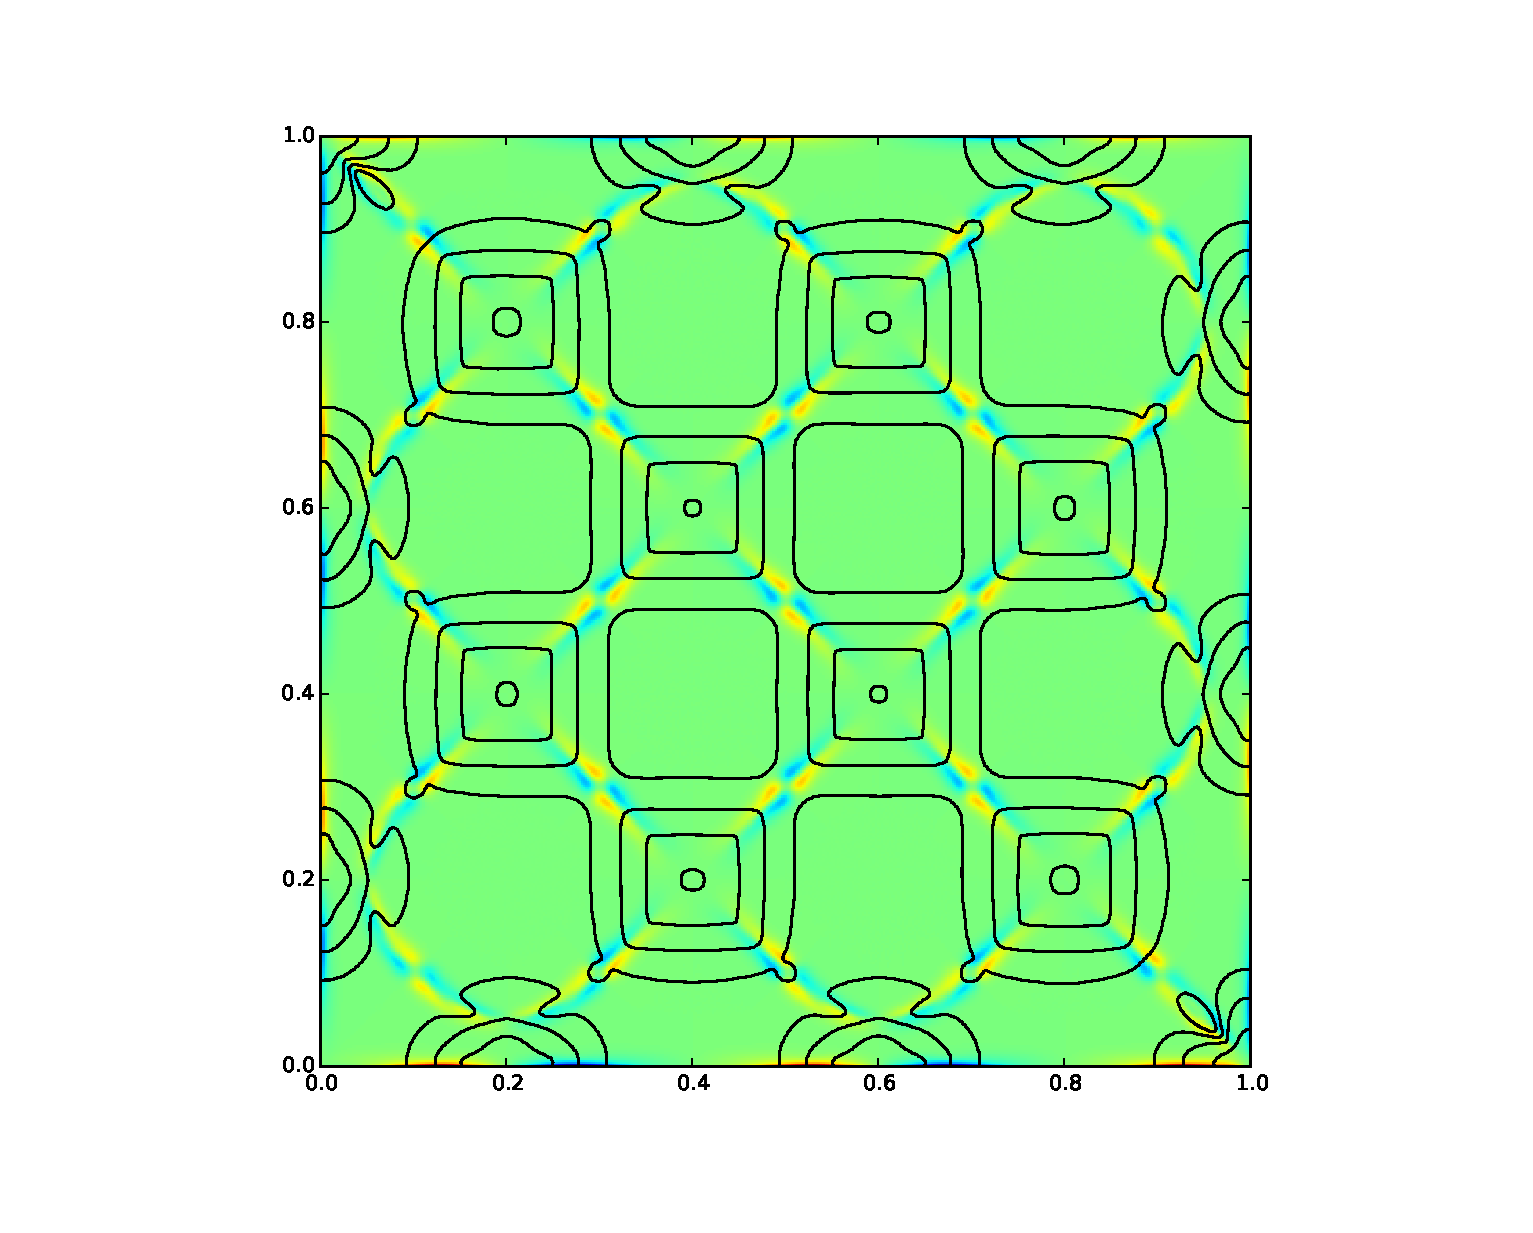
\includegraphics[width=\textwidth]{figs/vorticity-25-10}
\end{subfigure}
\begin{subfigure}[b]{0.32\textwidth}
  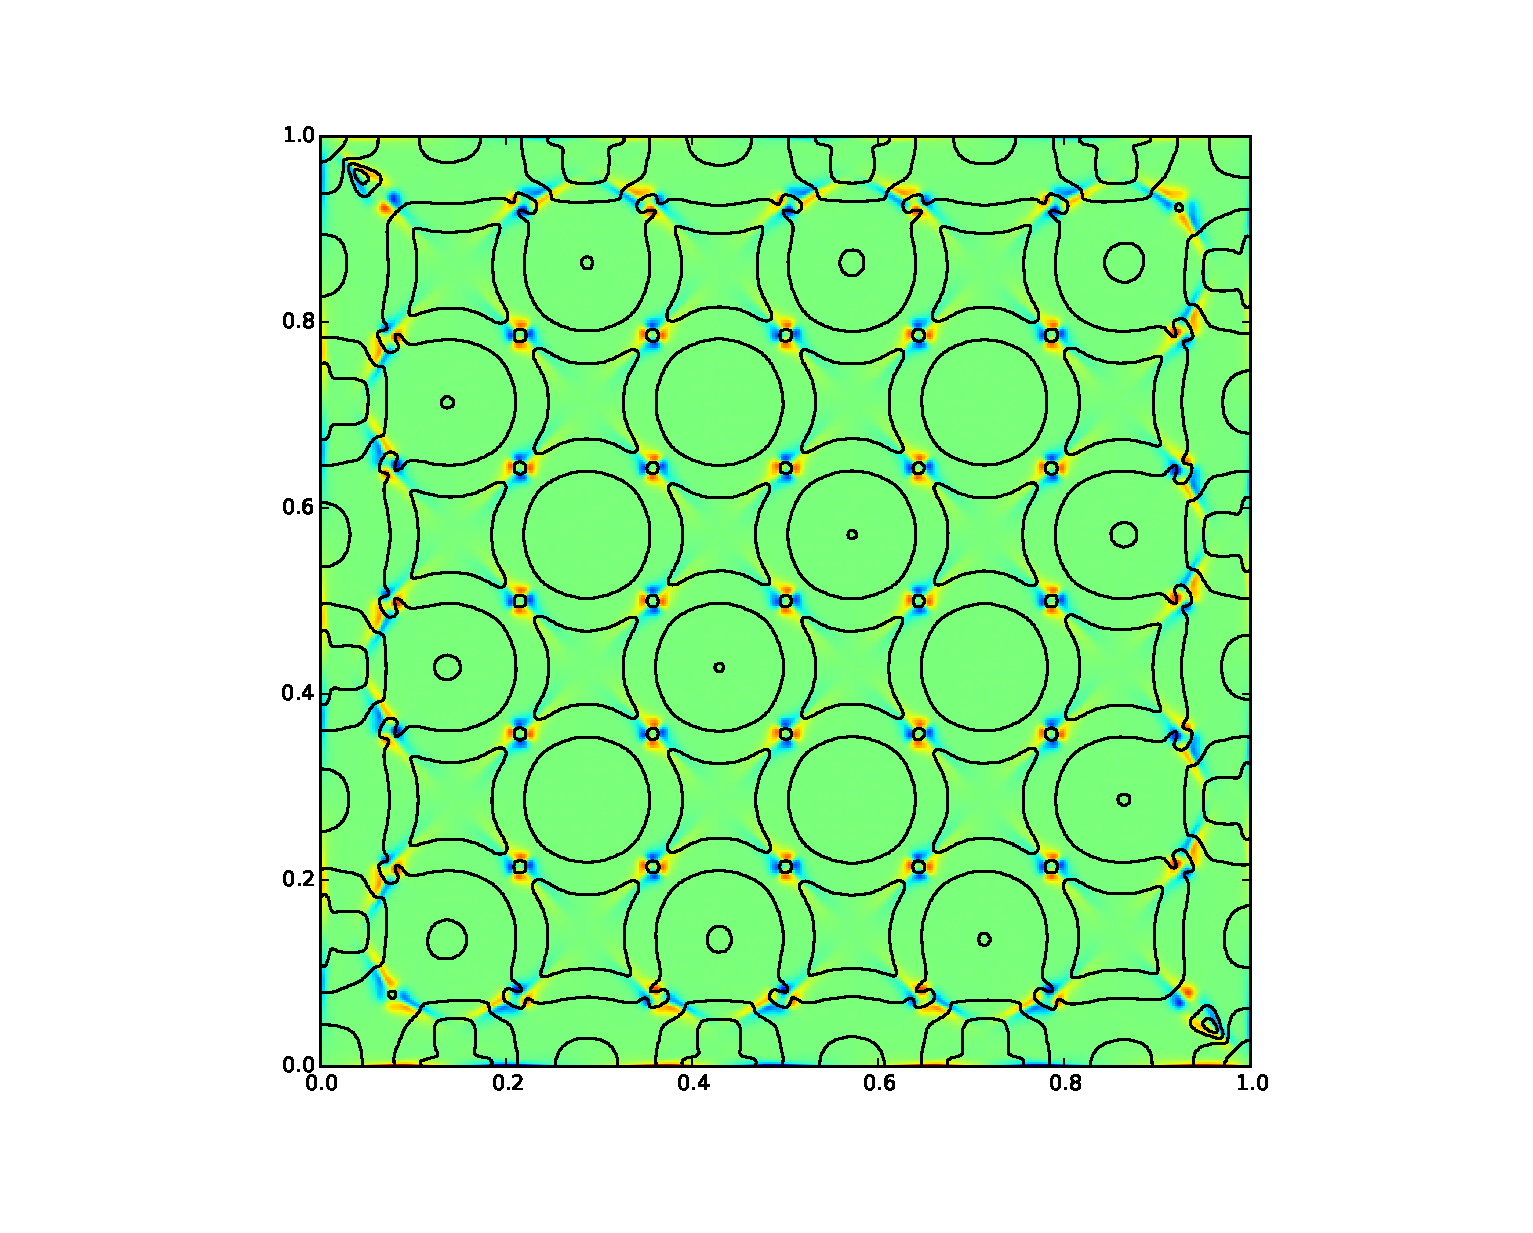
\includegraphics[width=\textwidth]{figs/vorticity-35-10}
\end{subfigure}
\begin{subfigure}[b]{0.32\textwidth}
  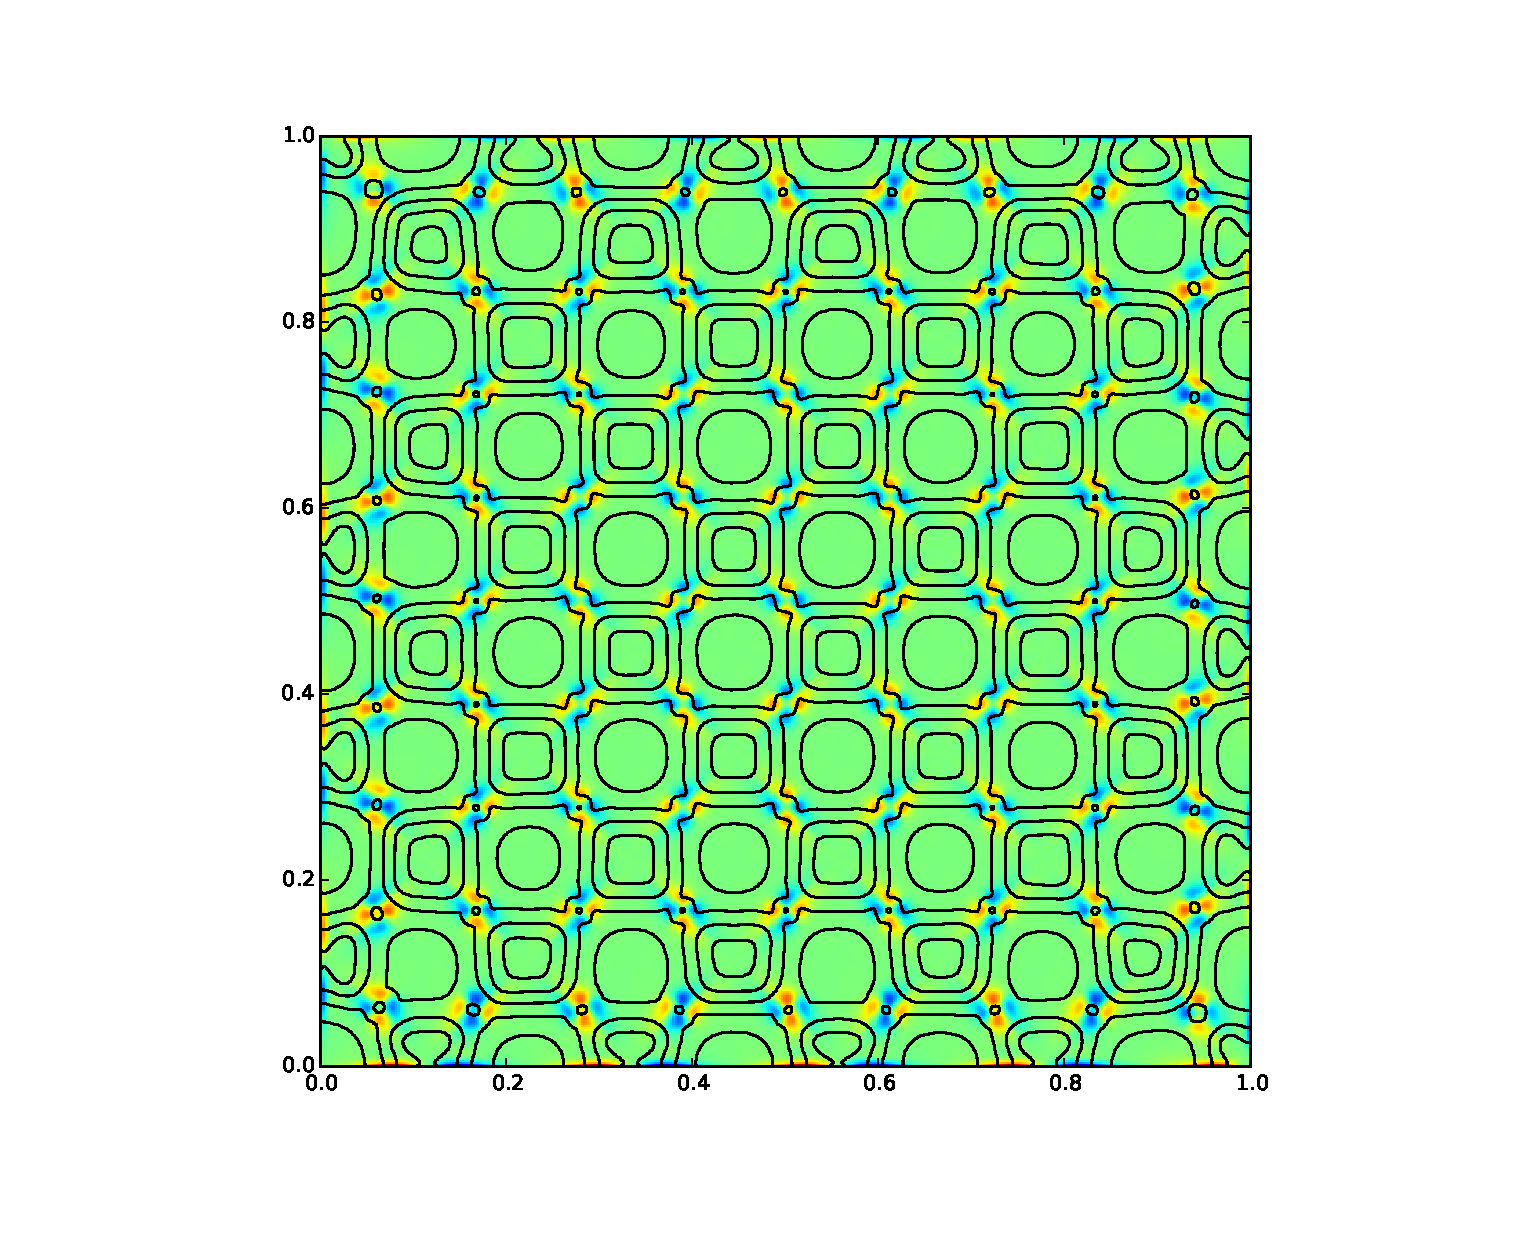
\includegraphics[width=\textwidth]{figs/vorticity-45-10}
\end{subfigure}
\caption{ \flabel{secondary}
Secondary flow in the horizontal mid-plane.
Background color is the vertical component of the vorticity.
Contours are lines of constant pressure.
}
\end{figure*}

\begin{figure*}
\begin{subfigure}[b]{0.32\textwidth}
  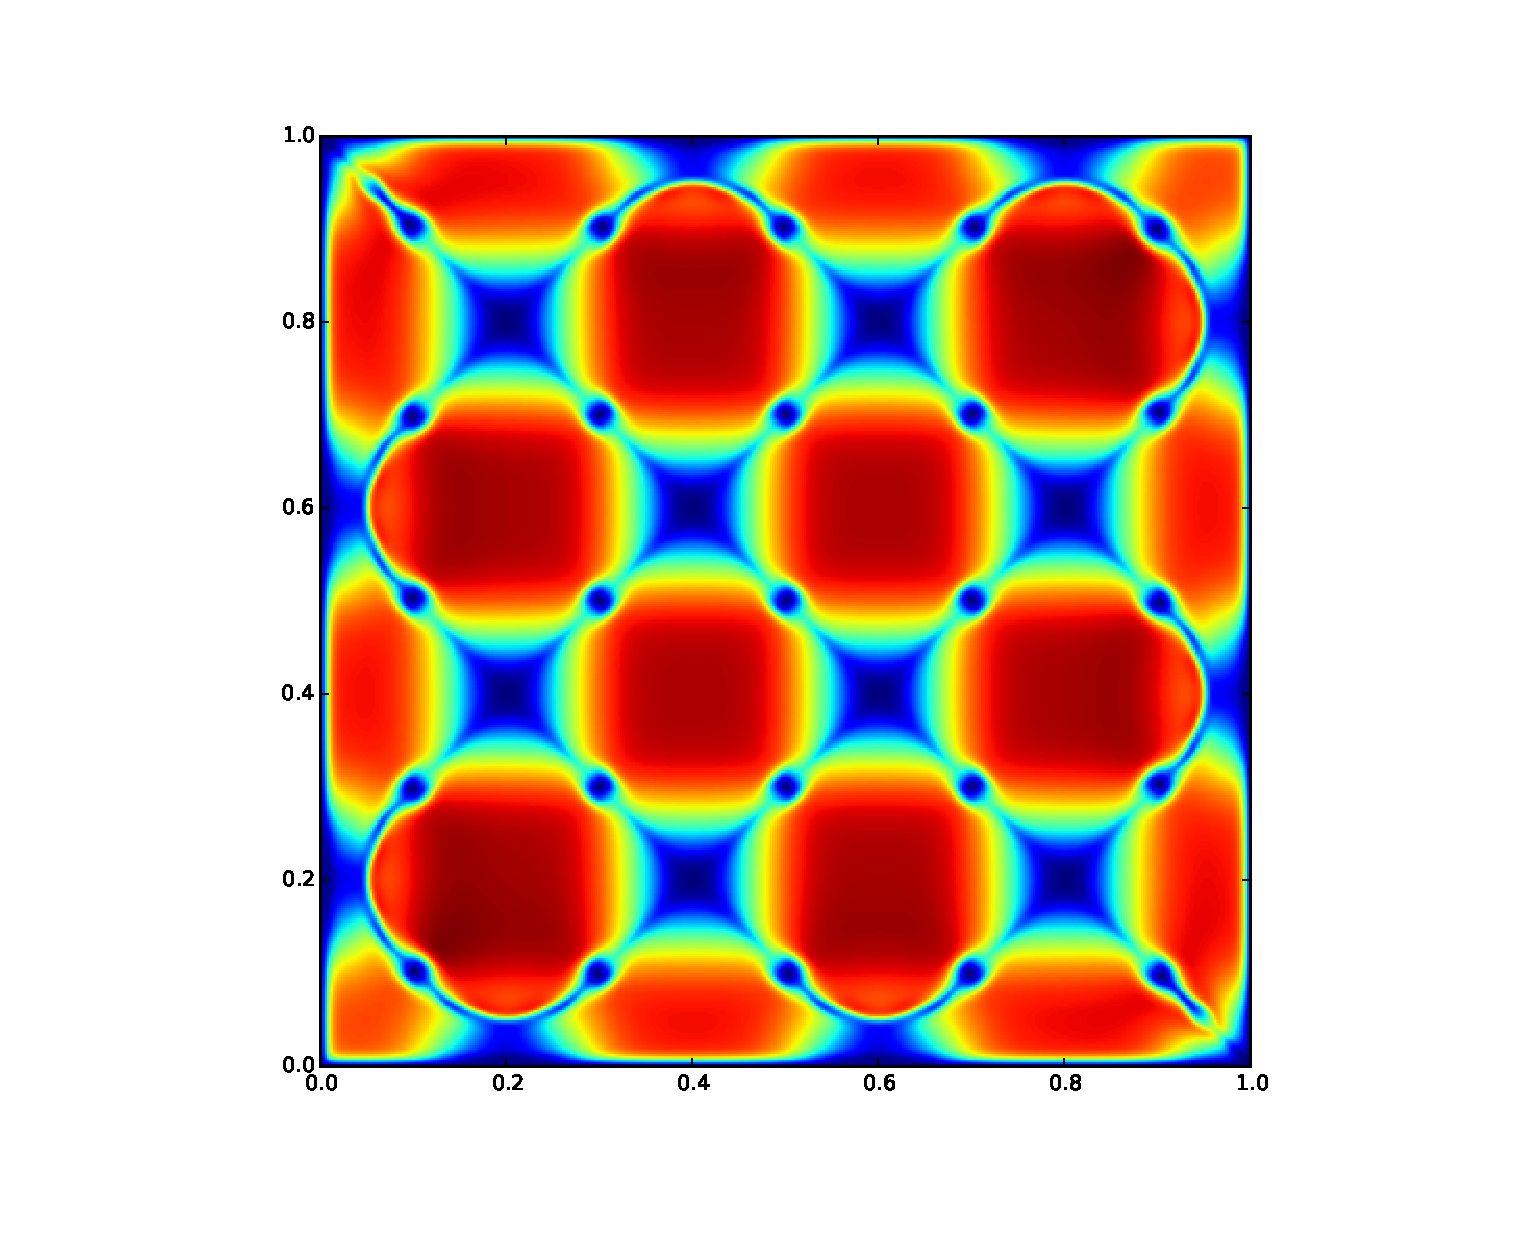
\includegraphics[width=\textwidth]{figs/dynamic_pressure-25-10}
\end{subfigure}
\begin{subfigure}[b]{0.32\textwidth}
  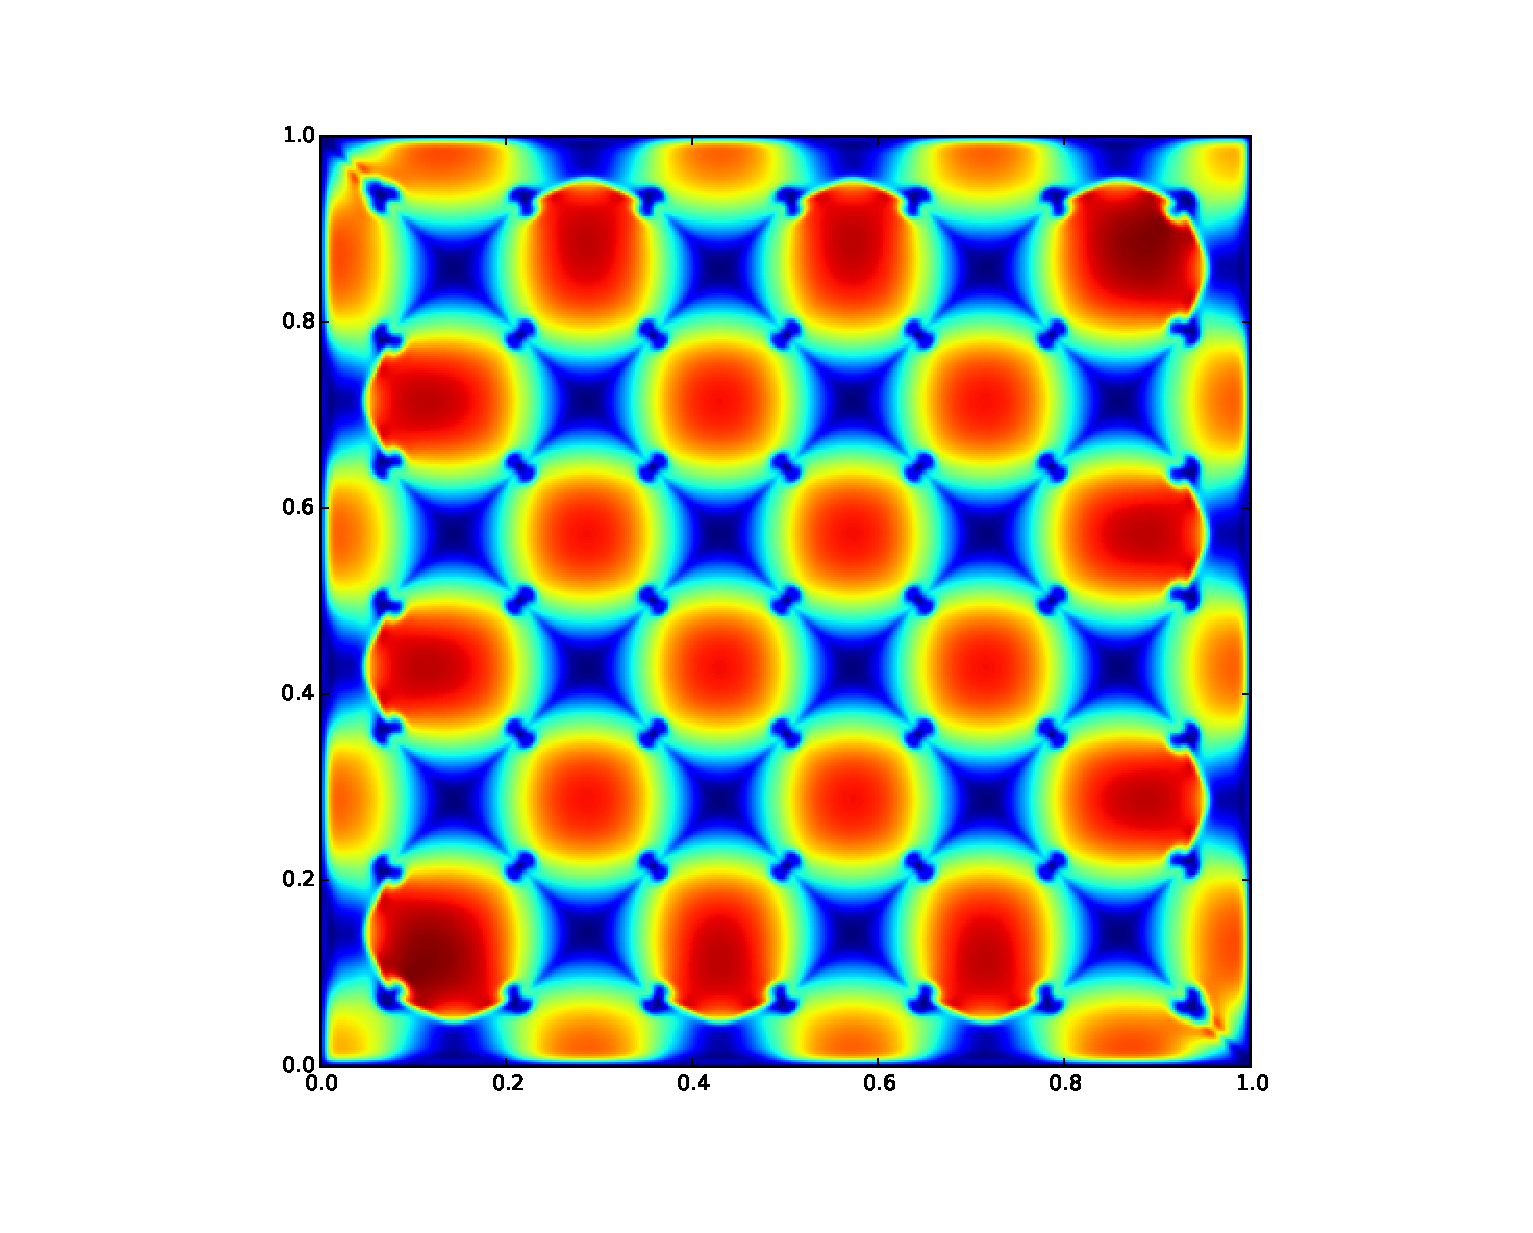
\includegraphics[width=\textwidth]{figs/dynamic_pressure-35-10}
\end{subfigure}
\begin{subfigure}[b]{0.32\textwidth}
  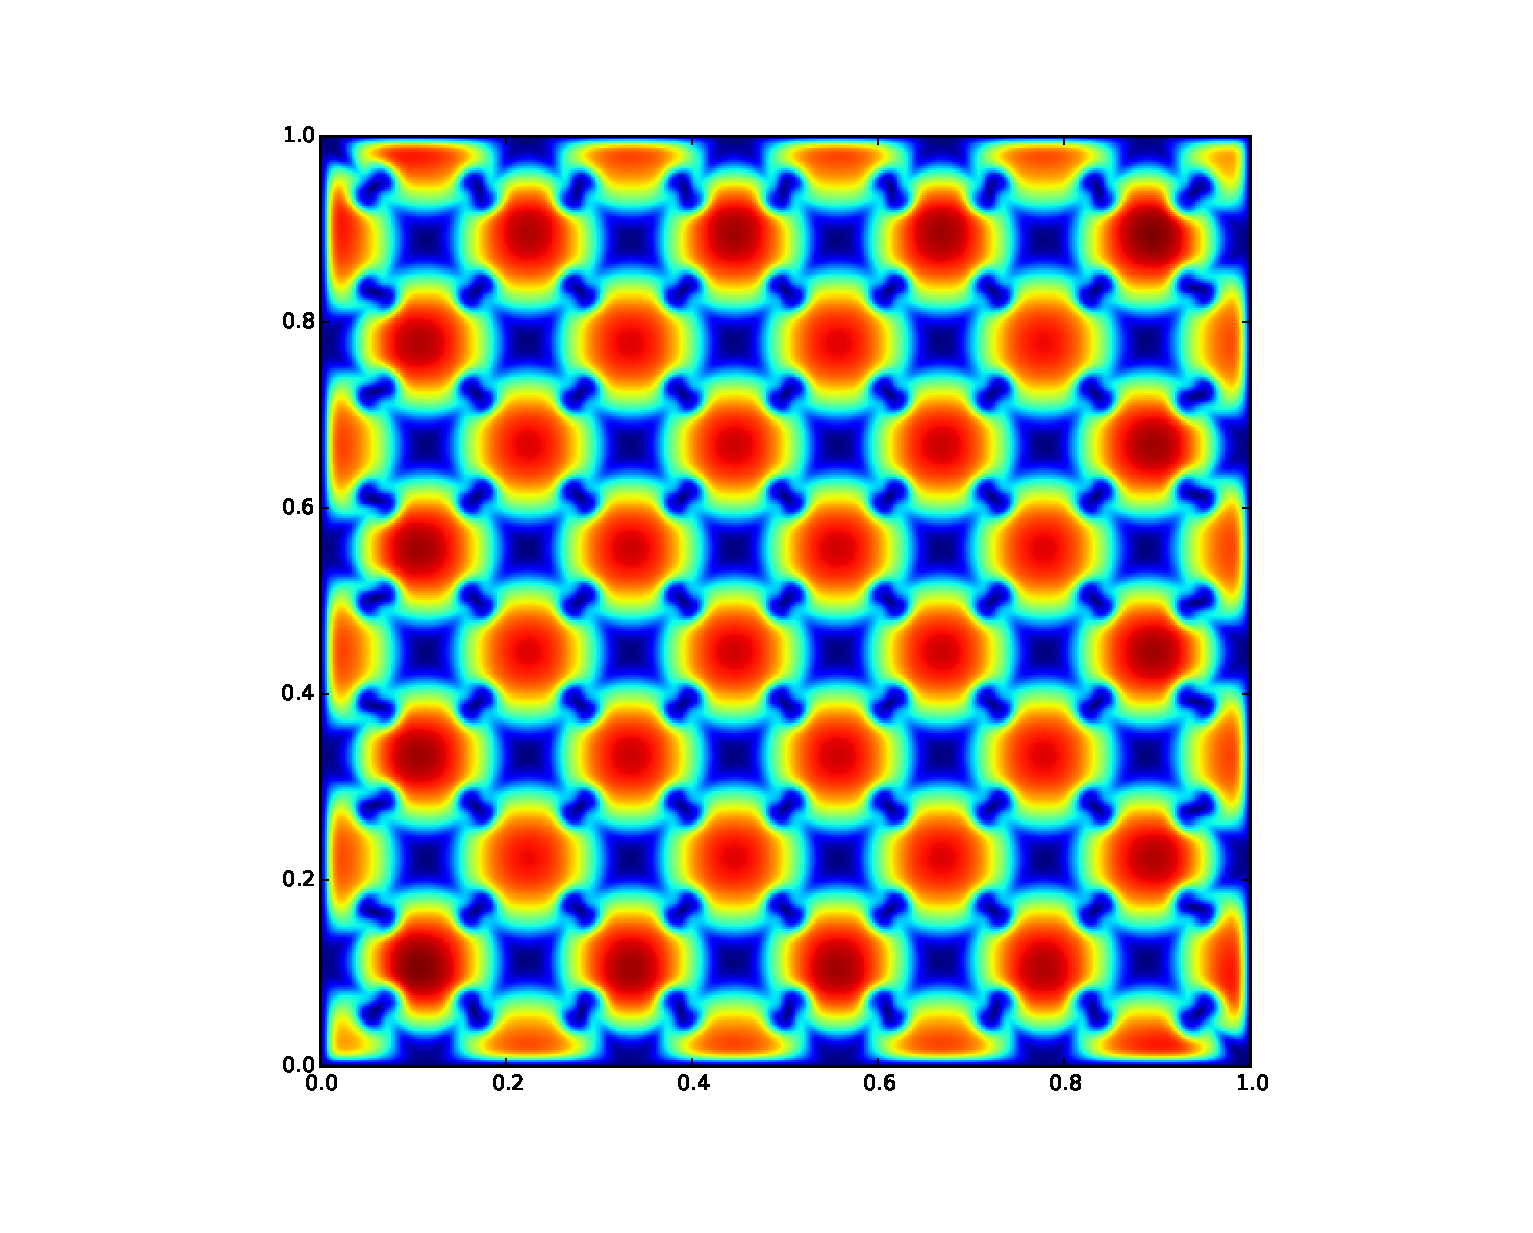
\includegraphics[width=\textwidth]{figs/dynamic_pressure-45-10}
\end{subfigure}
\caption{ \flabel{dynamic}
Dynamic pressure in the horizontal mid-plane.
}
\end{figure*}


In addition to the bubble height and vertical slices in the diagonal plane, we observe the horizontal mid-plane.
The span-wise scalar field, $\phi(x,y,0)$, exhibits plume structures that penetrate the bubble faces, as seen in \fref{phixy}.
The cause of these plumes is advection by secondary flows, as seen in \fref{secondary}.
Overlaying the pressure with the span-wise velocity reveals it to be secondary flow of the first kind: secondary flow due to span-wise pressure gradients.
The span-wise pressure gradient comes from the dynamic pressure of the rising and falling bubbles and spikes, in contrast to the stationary points at their interfaces.

The secondary flow advects mixed fluid from the interface into the centers of the bubbles and spikes.
Enhanced mixing reduces the effective Atwood number of the bubbles and spikes, but the magnitude of this effect is not clear.
As a secondary flow of the first kind, this mixing mode is present even at low Reynolds numbers.

